\documentclass[10pt]{article} % For LaTeX2e
\usepackage{tmlr}
% If accepted, instead use the following line for the camera-ready submission:
%\usepackage[accepted]{tmlr}
% To de-anonymize and remove mentions to TMLR (for example for posting to preprint servers), instead use the following:
%\usepackage[preprint]{tmlr}

% Optional math commands from https://github.com/goodfeli/dlbook_notation.
%%%%% NEW MATH DEFINITIONS %%%%%

\usepackage{amsmath,amsfonts,bm}

% Mark sections of captions for referring to divisions of figures
\newcommand{\figleft}{{\em (Left)}}
\newcommand{\figcenter}{{\em (Center)}}
\newcommand{\figright}{{\em (Right)}}
\newcommand{\figtop}{{\em (Top)}}
\newcommand{\figbottom}{{\em (Bottom)}}
\newcommand{\captiona}{{\em (a)}}
\newcommand{\captionb}{{\em (b)}}
\newcommand{\captionc}{{\em (c)}}
\newcommand{\captiond}{{\em (d)}}

% Highlight a newly defined term
\newcommand{\newterm}[1]{{\bf #1}}


% Figure reference, lower-case.
\def\figref#1{figure~\ref{#1}}
% Figure reference, capital. For start of sentence
\def\Figref#1{Figure~\ref{#1}}
\def\twofigref#1#2{figures \ref{#1} and \ref{#2}}
\def\quadfigref#1#2#3#4{figures \ref{#1}, \ref{#2}, \ref{#3} and \ref{#4}}
% Section reference, lower-case.
\def\secref#1{section~\ref{#1}}
% Section reference, capital.
\def\Secref#1{Section~\ref{#1}}
% Reference to two sections.
\def\twosecrefs#1#2{sections \ref{#1} and \ref{#2}}
% Reference to three sections.
\def\secrefs#1#2#3{sections \ref{#1}, \ref{#2} and \ref{#3}}
% Reference to an equation, lower-case.
\def\eqref#1{equation~\ref{#1}}
% Reference to an equation, upper case
\def\Eqref#1{Equation~\ref{#1}}
% A raw reference to an equation---avoid using if possible
\def\plaineqref#1{\ref{#1}}
% Reference to a chapter, lower-case.
\def\chapref#1{chapter~\ref{#1}}
% Reference to an equation, upper case.
\def\Chapref#1{Chapter~\ref{#1}}
% Reference to a range of chapters
\def\rangechapref#1#2{chapters\ref{#1}--\ref{#2}}
% Reference to an algorithm, lower-case.
\def\algref#1{algorithm~\ref{#1}}
% Reference to an algorithm, upper case.
\def\Algref#1{Algorithm~\ref{#1}}
\def\twoalgref#1#2{algorithms \ref{#1} and \ref{#2}}
\def\Twoalgref#1#2{Algorithms \ref{#1} and \ref{#2}}
% Reference to a part, lower case
\def\partref#1{part~\ref{#1}}
% Reference to a part, upper case
\def\Partref#1{Part~\ref{#1}}
\def\twopartref#1#2{parts \ref{#1} and \ref{#2}}

\def\ceil#1{\lceil #1 \rceil}
\def\floor#1{\lfloor #1 \rfloor}
\def\1{\bm{1}}
\newcommand{\train}{\mathcal{D}}
\newcommand{\valid}{\mathcal{D_{\mathrm{valid}}}}
\newcommand{\test}{\mathcal{D_{\mathrm{test}}}}

\def\eps{{\epsilon}}


% Random variables
\def\reta{{\textnormal{$\eta$}}}
\def\ra{{\textnormal{a}}}
\def\rb{{\textnormal{b}}}
\def\rc{{\textnormal{c}}}
\def\rd{{\textnormal{d}}}
\def\re{{\textnormal{e}}}
\def\rf{{\textnormal{f}}}
\def\rg{{\textnormal{g}}}
\def\rh{{\textnormal{h}}}
\def\ri{{\textnormal{i}}}
\def\rj{{\textnormal{j}}}
\def\rk{{\textnormal{k}}}
\def\rl{{\textnormal{l}}}
% rm is already a command, just don't name any random variables m
\def\rn{{\textnormal{n}}}
\def\ro{{\textnormal{o}}}
\def\rp{{\textnormal{p}}}
\def\rq{{\textnormal{q}}}
\def\rr{{\textnormal{r}}}
\def\rs{{\textnormal{s}}}
\def\rt{{\textnormal{t}}}
\def\ru{{\textnormal{u}}}
\def\rv{{\textnormal{v}}}
\def\rw{{\textnormal{w}}}
\def\rx{{\textnormal{x}}}
\def\ry{{\textnormal{y}}}
\def\rz{{\textnormal{z}}}

% Random vectors
\def\rvepsilon{{\mathbf{\epsilon}}}
\def\rvtheta{{\mathbf{\theta}}}
\def\rva{{\mathbf{a}}}
\def\rvb{{\mathbf{b}}}
\def\rvc{{\mathbf{c}}}
\def\rvd{{\mathbf{d}}}
\def\rve{{\mathbf{e}}}
\def\rvf{{\mathbf{f}}}
\def\rvg{{\mathbf{g}}}
\def\rvh{{\mathbf{h}}}
\def\rvu{{\mathbf{i}}}
\def\rvj{{\mathbf{j}}}
\def\rvk{{\mathbf{k}}}
\def\rvl{{\mathbf{l}}}
\def\rvm{{\mathbf{m}}}
\def\rvn{{\mathbf{n}}}
\def\rvo{{\mathbf{o}}}
\def\rvp{{\mathbf{p}}}
\def\rvq{{\mathbf{q}}}
\def\rvr{{\mathbf{r}}}
\def\rvs{{\mathbf{s}}}
\def\rvt{{\mathbf{t}}}
\def\rvu{{\mathbf{u}}}
\def\rvv{{\mathbf{v}}}
\def\rvw{{\mathbf{w}}}
\def\rvx{{\mathbf{x}}}
\def\rvy{{\mathbf{y}}}
\def\rvz{{\mathbf{z}}}

% Elements of random vectors
\def\erva{{\textnormal{a}}}
\def\ervb{{\textnormal{b}}}
\def\ervc{{\textnormal{c}}}
\def\ervd{{\textnormal{d}}}
\def\erve{{\textnormal{e}}}
\def\ervf{{\textnormal{f}}}
\def\ervg{{\textnormal{g}}}
\def\ervh{{\textnormal{h}}}
\def\ervi{{\textnormal{i}}}
\def\ervj{{\textnormal{j}}}
\def\ervk{{\textnormal{k}}}
\def\ervl{{\textnormal{l}}}
\def\ervm{{\textnormal{m}}}
\def\ervn{{\textnormal{n}}}
\def\ervo{{\textnormal{o}}}
\def\ervp{{\textnormal{p}}}
\def\ervq{{\textnormal{q}}}
\def\ervr{{\textnormal{r}}}
\def\ervs{{\textnormal{s}}}
\def\ervt{{\textnormal{t}}}
\def\ervu{{\textnormal{u}}}
\def\ervv{{\textnormal{v}}}
\def\ervw{{\textnormal{w}}}
\def\ervx{{\textnormal{x}}}
\def\ervy{{\textnormal{y}}}
\def\ervz{{\textnormal{z}}}

% Random matrices
\def\rmA{{\mathbf{A}}}
\def\rmB{{\mathbf{B}}}
\def\rmC{{\mathbf{C}}}
\def\rmD{{\mathbf{D}}}
\def\rmE{{\mathbf{E}}}
\def\rmF{{\mathbf{F}}}
\def\rmG{{\mathbf{G}}}
\def\rmH{{\mathbf{H}}}
\def\rmI{{\mathbf{I}}}
\def\rmJ{{\mathbf{J}}}
\def\rmK{{\mathbf{K}}}
\def\rmL{{\mathbf{L}}}
\def\rmM{{\mathbf{M}}}
\def\rmN{{\mathbf{N}}}
\def\rmO{{\mathbf{O}}}
\def\rmP{{\mathbf{P}}}
\def\rmQ{{\mathbf{Q}}}
\def\rmR{{\mathbf{R}}}
\def\rmS{{\mathbf{S}}}
\def\rmT{{\mathbf{T}}}
\def\rmU{{\mathbf{U}}}
\def\rmV{{\mathbf{V}}}
\def\rmW{{\mathbf{W}}}
\def\rmX{{\mathbf{X}}}
\def\rmY{{\mathbf{Y}}}
\def\rmZ{{\mathbf{Z}}}

% Elements of random matrices
\def\ermA{{\textnormal{A}}}
\def\ermB{{\textnormal{B}}}
\def\ermC{{\textnormal{C}}}
\def\ermD{{\textnormal{D}}}
\def\ermE{{\textnormal{E}}}
\def\ermF{{\textnormal{F}}}
\def\ermG{{\textnormal{G}}}
\def\ermH{{\textnormal{H}}}
\def\ermI{{\textnormal{I}}}
\def\ermJ{{\textnormal{J}}}
\def\ermK{{\textnormal{K}}}
\def\ermL{{\textnormal{L}}}
\def\ermM{{\textnormal{M}}}
\def\ermN{{\textnormal{N}}}
\def\ermO{{\textnormal{O}}}
\def\ermP{{\textnormal{P}}}
\def\ermQ{{\textnormal{Q}}}
\def\ermR{{\textnormal{R}}}
\def\ermS{{\textnormal{S}}}
\def\ermT{{\textnormal{T}}}
\def\ermU{{\textnormal{U}}}
\def\ermV{{\textnormal{V}}}
\def\ermW{{\textnormal{W}}}
\def\ermX{{\textnormal{X}}}
\def\ermY{{\textnormal{Y}}}
\def\ermZ{{\textnormal{Z}}}

% Vectors
\def\vzero{{\bm{0}}}
\def\vone{{\bm{1}}}
\def\vmu{{\bm{\mu}}}
\def\vtheta{{\bm{\theta}}}
\def\va{{\bm{a}}}
\def\vb{{\bm{b}}}
\def\vc{{\bm{c}}}
\def\vd{{\bm{d}}}
\def\ve{{\bm{e}}}
\def\vf{{\bm{f}}}
\def\vg{{\bm{g}}}
\def\vh{{\bm{h}}}
\def\vi{{\bm{i}}}
\def\vj{{\bm{j}}}
\def\vk{{\bm{k}}}
\def\vl{{\bm{l}}}
\def\vm{{\bm{m}}}
\def\vn{{\bm{n}}}
\def\vo{{\bm{o}}}
\def\vp{{\bm{p}}}
\def\vq{{\bm{q}}}
\def\vr{{\bm{r}}}
\def\vs{{\bm{s}}}
\def\vt{{\bm{t}}}
\def\vu{{\bm{u}}}
\def\vv{{\bm{v}}}
\def\vw{{\bm{w}}}
\def\vx{{\bm{x}}}
\def\vy{{\bm{y}}}
\def\vz{{\bm{z}}}

% Elements of vectors
\def\evalpha{{\alpha}}
\def\evbeta{{\beta}}
\def\evepsilon{{\epsilon}}
\def\evlambda{{\lambda}}
\def\evomega{{\omega}}
\def\evmu{{\mu}}
\def\evpsi{{\psi}}
\def\evsigma{{\sigma}}
\def\evtheta{{\theta}}
\def\eva{{a}}
\def\evb{{b}}
\def\evc{{c}}
\def\evd{{d}}
\def\eve{{e}}
\def\evf{{f}}
\def\evg{{g}}
\def\evh{{h}}
\def\evi{{i}}
\def\evj{{j}}
\def\evk{{k}}
\def\evl{{l}}
\def\evm{{m}}
\def\evn{{n}}
\def\evo{{o}}
\def\evp{{p}}
\def\evq{{q}}
\def\evr{{r}}
\def\evs{{s}}
\def\evt{{t}}
\def\evu{{u}}
\def\evv{{v}}
\def\evw{{w}}
\def\evx{{x}}
\def\evy{{y}}
\def\evz{{z}}

% Matrix
\def\mA{{\bm{A}}}
\def\mB{{\bm{B}}}
\def\mC{{\bm{C}}}
\def\mD{{\bm{D}}}
\def\mE{{\bm{E}}}
\def\mF{{\bm{F}}}
\def\mG{{\bm{G}}}
\def\mH{{\bm{H}}}
\def\mI{{\bm{I}}}
\def\mJ{{\bm{J}}}
\def\mK{{\bm{K}}}
\def\mL{{\bm{L}}}
\def\mM{{\bm{M}}}
\def\mN{{\bm{N}}}
\def\mO{{\bm{O}}}
\def\mP{{\bm{P}}}
\def\mQ{{\bm{Q}}}
\def\mR{{\bm{R}}}
\def\mS{{\bm{S}}}
\def\mT{{\bm{T}}}
\def\mU{{\bm{U}}}
\def\mV{{\bm{V}}}
\def\mW{{\bm{W}}}
\def\mX{{\bm{X}}}
\def\mY{{\bm{Y}}}
\def\mZ{{\bm{Z}}}
\def\mBeta{{\bm{\beta}}}
\def\mPhi{{\bm{\Phi}}}
\def\mLambda{{\bm{\Lambda}}}
\def\mSigma{{\bm{\Sigma}}}

% Tensor
\DeclareMathAlphabet{\mathsfit}{\encodingdefault}{\sfdefault}{m}{sl}
\SetMathAlphabet{\mathsfit}{bold}{\encodingdefault}{\sfdefault}{bx}{n}
\newcommand{\tens}[1]{\bm{\mathsfit{#1}}}
\def\tA{{\tens{A}}}
\def\tB{{\tens{B}}}
\def\tC{{\tens{C}}}
\def\tD{{\tens{D}}}
\def\tE{{\tens{E}}}
\def\tF{{\tens{F}}}
\def\tG{{\tens{G}}}
\def\tH{{\tens{H}}}
\def\tI{{\tens{I}}}
\def\tJ{{\tens{J}}}
\def\tK{{\tens{K}}}
\def\tL{{\tens{L}}}
\def\tM{{\tens{M}}}
\def\tN{{\tens{N}}}
\def\tO{{\tens{O}}}
\def\tP{{\tens{P}}}
\def\tQ{{\tens{Q}}}
\def\tR{{\tens{R}}}
\def\tS{{\tens{S}}}
\def\tT{{\tens{T}}}
\def\tU{{\tens{U}}}
\def\tV{{\tens{V}}}
\def\tW{{\tens{W}}}
\def\tX{{\tens{X}}}
\def\tY{{\tens{Y}}}
\def\tZ{{\tens{Z}}}


% Graph
\def\gA{{\mathcal{A}}}
\def\gB{{\mathcal{B}}}
\def\gC{{\mathcal{C}}}
\def\gD{{\mathcal{D}}}
\def\gE{{\mathcal{E}}}
\def\gF{{\mathcal{F}}}
\def\gG{{\mathcal{G}}}
\def\gH{{\mathcal{H}}}
\def\gI{{\mathcal{I}}}
\def\gJ{{\mathcal{J}}}
\def\gK{{\mathcal{K}}}
\def\gL{{\mathcal{L}}}
\def\gM{{\mathcal{M}}}
\def\gN{{\mathcal{N}}}
\def\gO{{\mathcal{O}}}
\def\gP{{\mathcal{P}}}
\def\gQ{{\mathcal{Q}}}
\def\gR{{\mathcal{R}}}
\def\gS{{\mathcal{S}}}
\def\gT{{\mathcal{T}}}
\def\gU{{\mathcal{U}}}
\def\gV{{\mathcal{V}}}
\def\gW{{\mathcal{W}}}
\def\gX{{\mathcal{X}}}
\def\gY{{\mathcal{Y}}}
\def\gZ{{\mathcal{Z}}}

% Sets
\def\sA{{\mathbb{A}}}
\def\sB{{\mathbb{B}}}
\def\sC{{\mathbb{C}}}
\def\sD{{\mathbb{D}}}
% Don't use a set called E, because this would be the same as our symbol
% for expectation.
\def\sF{{\mathbb{F}}}
\def\sG{{\mathbb{G}}}
\def\sH{{\mathbb{H}}}
\def\sI{{\mathbb{I}}}
\def\sJ{{\mathbb{J}}}
\def\sK{{\mathbb{K}}}
\def\sL{{\mathbb{L}}}
\def\sM{{\mathbb{M}}}
\def\sN{{\mathbb{N}}}
\def\sO{{\mathbb{O}}}
\def\sP{{\mathbb{P}}}
\def\sQ{{\mathbb{Q}}}
\def\sR{{\mathbb{R}}}
\def\sS{{\mathbb{S}}}
\def\sT{{\mathbb{T}}}
\def\sU{{\mathbb{U}}}
\def\sV{{\mathbb{V}}}
\def\sW{{\mathbb{W}}}
\def\sX{{\mathbb{X}}}
\def\sY{{\mathbb{Y}}}
\def\sZ{{\mathbb{Z}}}

% Entries of a matrix
\def\emLambda{{\Lambda}}
\def\emA{{A}}
\def\emB{{B}}
\def\emC{{C}}
\def\emD{{D}}
\def\emE{{E}}
\def\emF{{F}}
\def\emG{{G}}
\def\emH{{H}}
\def\emI{{I}}
\def\emJ{{J}}
\def\emK{{K}}
\def\emL{{L}}
\def\emM{{M}}
\def\emN{{N}}
\def\emO{{O}}
\def\emP{{P}}
\def\emQ{{Q}}
\def\emR{{R}}
\def\emS{{S}}
\def\emT{{T}}
\def\emU{{U}}
\def\emV{{V}}
\def\emW{{W}}
\def\emX{{X}}
\def\emY{{Y}}
\def\emZ{{Z}}
\def\emSigma{{\Sigma}}

% entries of a tensor
% Same font as tensor, without \bm wrapper
\newcommand{\etens}[1]{\mathsfit{#1}}
\def\etLambda{{\etens{\Lambda}}}
\def\etA{{\etens{A}}}
\def\etB{{\etens{B}}}
\def\etC{{\etens{C}}}
\def\etD{{\etens{D}}}
\def\etE{{\etens{E}}}
\def\etF{{\etens{F}}}
\def\etG{{\etens{G}}}
\def\etH{{\etens{H}}}
\def\etI{{\etens{I}}}
\def\etJ{{\etens{J}}}
\def\etK{{\etens{K}}}
\def\etL{{\etens{L}}}
\def\etM{{\etens{M}}}
\def\etN{{\etens{N}}}
\def\etO{{\etens{O}}}
\def\etP{{\etens{P}}}
\def\etQ{{\etens{Q}}}
\def\etR{{\etens{R}}}
\def\etS{{\etens{S}}}
\def\etT{{\etens{T}}}
\def\etU{{\etens{U}}}
\def\etV{{\etens{V}}}
\def\etW{{\etens{W}}}
\def\etX{{\etens{X}}}
\def\etY{{\etens{Y}}}
\def\etZ{{\etens{Z}}}

% The true underlying data generating distribution
\newcommand{\pdata}{p_{\rm{data}}}
% The empirical distribution defined by the training set
\newcommand{\ptrain}{\hat{p}_{\rm{data}}}
\newcommand{\Ptrain}{\hat{P}_{\rm{data}}}
% The model distribution
\newcommand{\pmodel}{p_{\rm{model}}}
\newcommand{\Pmodel}{P_{\rm{model}}}
\newcommand{\ptildemodel}{\tilde{p}_{\rm{model}}}
% Stochastic autoencoder distributions
\newcommand{\pencode}{p_{\rm{encoder}}}
\newcommand{\pdecode}{p_{\rm{decoder}}}
\newcommand{\precons}{p_{\rm{reconstruct}}}

\newcommand{\laplace}{\mathrm{Laplace}} % Laplace distribution

\newcommand{\E}{\mathbb{E}}
\newcommand{\Ls}{\mathcal{L}}
\newcommand{\R}{\mathbb{R}}
\newcommand{\emp}{\tilde{p}}
\newcommand{\lr}{\alpha}
\newcommand{\reg}{\lambda}
\newcommand{\rect}{\mathrm{rectifier}}
\newcommand{\softmax}{\mathrm{softmax}}
\newcommand{\sigmoid}{\sigma}
\newcommand{\softplus}{\zeta}
\newcommand{\KL}{D_{\mathrm{KL}}}
\newcommand{\Var}{\mathrm{Var}}
\newcommand{\standarderror}{\mathrm{SE}}
\newcommand{\Cov}{\mathrm{Cov}}
% Wolfram Mathworld says $L^2$ is for function spaces and $\ell^2$ is for vectors
% But then they seem to use $L^2$ for vectors throughout the site, and so does
% wikipedia.
\newcommand{\normlzero}{L^0}
\newcommand{\normlone}{L^1}
\newcommand{\normltwo}{L^2}
\newcommand{\normlp}{L^p}
\newcommand{\normmax}{L^\infty}

\newcommand{\parents}{Pa} % See usage in notation.tex. Chosen to match Daphne's book.

\DeclareMathOperator*{\argmax}{arg\,max}
\DeclareMathOperator*{\argmin}{arg\,min}

\DeclareMathOperator{\sign}{sign}
\DeclareMathOperator{\Tr}{Tr}
\let\ab\allowbreak


\usepackage{amsmath}
\usepackage{amssymb}
\usepackage{booktabs}
\usepackage{placeins}
\usepackage{array}
\usepackage{graphicx}
\usepackage{fancyvrb}
\usepackage{seqsplit}
\usepackage{hyperref}
\usepackage{url}

% Unicode characters used throughout the tables and text.
\DeclareUnicodeCharacter{2212}{\ensuremath{-}}
\DeclareUnicodeCharacter{00D7}{\ensuremath{\times}}

% Literal prompt text, candidate values, and identifiers.
\newcommand{\lit}[1]{\texttt{#1}}
% Prompt examples.
\DefineVerbatimEnvironment{prompt}{Verbatim}{frame=single,fontsize=\small,xleftmargin=1em,xrightmargin=1em}

\title{What a Stale Value Still Does: Mention Structure and Order\\Shape Score Sensitivity After In-Context Updates}

% Authors must not appear in the submitted version. They should be hidden
% as long as the tmlr package is used without the [accepted] or [preprint] options.
% Non-anonymous submissions will be rejected without review.

\author{\name Anonymous Authors \email anonymous@example.com \\
      \addr Anonymous Institution}

\def\month{MM}  % Insert correct month for camera-ready version
\def\year{YYYY} % Insert correct year for camera-ready version
\def\openreview{\url{https://openreview.net/forum?id=XXXX}} % Insert correct link to OpenReview for camera-ready version


\begin{document}

\maketitle

{\renewcommand{\thefootnote}{}\footnotetext{A large language model assisted with drafting and revision of this manuscript. The authors are responsible for checking the accuracy of its claims, analyses, references, and final text.}}

\begin{abstract}
When a context updates a fact, does the earlier value still shape a model's answer scores? We replace a historical value in two-entity histories, keeping current assignments fixed, and measure how much more this shifts candidate scores for a query about the associated entity than about the other entity. Across six prompt constructions crossed with mention order in Qwen3-8B and Gemma 3 4B, this sensitivity depends more on how and where the value is mentioned than on whether it was ever assigned to the queried attribute. Whether the updated value belonged to the queried attribute or another one changes sensitivity on average by only 0.314 nats in Qwen and 0.004 in Gemma. A value mentioned in a note about the entity outweighs a superseded assignment; with the marker \lit{Previously} and the distance between name and value matched, the difference is 1.293 and 0.367 nats. Never-assigned values are credited to whichever entity shares their position, and \lit{Previously} lowers sensitivity, but how order and the marker interact with construction differs between models. These are bounded candidate scores from models that rank the current value first; in an exploratory study of a below-ceiling model, generated answers follow the same pattern.
\end{abstract}

\section{Introduction}
\label{sec:introduction}

Conversations and documents often update a fact while leaving its earlier version in view. A user's preference changes, an object moves, a task variable receives a new value. A language model can answer with the current value and still be influenced by the old one: its scores for candidate answers may shift when the old value changes, even though the top answer does not. This paper asks what governs that residual sensitivity.

Consider a history from our main experiment:

\begin{prompt}
Previously, Nora’s badge was amber.
Previously, Liam’s badge was coral.
Currently, Nora’s badge is jade.
Currently, Liam’s badge is pearl.
What is Nora’s current badge?
Respond with only the value, with no explanation.
\end{prompt}

The correct answer is \lit{jade}. Suppose we replace the earlier \lit{amber} with \lit{violet} and leave everything else unchanged. The edit can shift the model's scores for \lit{violet} relative to \lit{amber}. If the shift is larger when the question asks about Nora than when it asks about Liam, the old value carries information that is specific to Nora. We call the difference between these two shifts \emph{query relevance}, $R$ (Section~\ref{sec:edits}).

A positive $R$ for the history above could arise for several reasons. The model may represent that \lit{amber} \emph{was} Nora's badge---a superseded assignment to the queried attribute. It may simply associate \lit{amber} with Nora because the two appear in the same sentence. Or it may link \lit{amber} to Nora by position, because both come first in their blocks. The marker \lit{Previously} could also change how much weight the old value receives. We separate these accounts with prompt constructions that hold some of these properties fixed while varying others, and we cross every construction with the order in which the entities appear in the historical and current blocks.

The answer is consistent across the two models we test, Qwen3-8B and Gemma 3 4B: \textbf{query-specific score sensitivity to a historical value is governed by surface association---mention construction, relative position, and temporal marking---and only weakly by whether the value was ever assigned to the queried attribute.} Whether the earlier value belonged to the queried attribute and was then updated, or belonged to a different attribute that was never updated, with the sentence otherwise identical, moves $R$ by about a third of a nat in Qwen and not detectably in Gemma. Mentioning the value in a note about the entity instead of assigning it raises $R$ by several nats. Values that are mentioned but assigned to no one inherit the entity that occupies the same relative position, so their effect reverses sign when the order of mentions is reversed. And the marker \lit{Previously} lowers $R$ wherever it is added.

Our contributions are:
\begin{enumerate}
\item A counterfactual measure of query-specific sensitivity to a historical value, applied to six prompt constructions crossed with independently varied historical and current mention order (Sections~\ref{sec:task}--\ref{sec:setup}).
\item A decomposition showing that relation status contributes little to this sensitivity, whereas construction, relative position, and temporal marking each change it by nats (Section~\ref{sec:main-findings}, Figure~\ref{fig:decomposition}).
\item Evidence of position-based association: never-assigned values raise relevance for the entity in the matching position and lower it for the other, effects that cancel when orders are averaged (Section~\ref{sec:order}).
\item A controlled test of the temporal marker \lit{Previously}, which lowers relevance in superseded and entity-mention constructions in both models; the gap between the two constructions persists without the marker, which motivates a name--value proximity hypothesis for future tests (Sections~\ref{sec:marker-results} and~\ref{sec:discussion}).
\end{enumerate}

\section{Related work}
\label{sec:related}

\paragraph{Contextual updates and knowledge conflicts.} Entity-tracking benchmarks test whether models recover an entity's state after a sequence of operations \citep{kim2023entity,tang2026entities}, and belief-revision and in-context forgetting studies test whether models revise conclusions or stop using information once new evidence or instructions arrive \citep{wilie2024belief,qian2026forget}. \citet{wang2025unable} show that earlier key--value updates interfere with retrieving the latest value as the number of updates grows, and \citet{guo2026context} characterize stale-answer failures after context updates, including whether the current value remains recoverable and how attention drifts during answer selection. More broadly, \citet{xu2024conflicts} survey knowledge conflicts and distinguish conflicts between context and parametric memory, within the context, and within memory; contradictions between earlier and later statements in a single context belong to the second type. \citet{yang2026conflicts} study such intra-context conflicts and report a consistent bias toward earlier evidence. These studies measure whether the final answer is correct; we ask how an earlier value influences scores when the answer is already right, and which properties of its mention carry that influence.

\paragraph{Position in context.} Where information sits in the context affects how models use it. \citet{liu2024lost} show that retrieval accuracy depends strongly on the position of the relevant passage in long inputs, and \citet{yang2026conflicts} identify a positional preference as an obstacle to resolving conflicts. Our contexts are six lines long, far from the long-context regime, yet relative position still determines which entity a never-assigned value is credited to.

\paragraph{Entity binding.} Mechanistic studies analyze how models bind entities to attributes in context and retrieve those bindings, including binding-ID representations \citep{feng2024bind}, mixtures of positional, lexical, and reflexive retrieval mechanisms \citep{gurarieh2026mixing}, and lookback mechanisms for tracking characters' beliefs \citep{prakash2026lookbacks}. These works intervene on internal activations. We work at the level of prompts and output scores, which lets us compare how different surface constructions feed whatever binding mechanism the model uses, but not identify the mechanism itself.

\paragraph{Persistence after knowledge editing.} Knowledge-editing studies ask what remains of a fact after a model's parametric knowledge is changed: whether original facts stay linearly decodable after an edit \citep{srivastava2026suppressed} and whether they resurface after superficially successful edits \citep{xie2025deceptiveness}. In our setting both the earlier and the current value are present in the input and the model is not edited; we measure sensitivity to an earlier value that is still in view.

\section{Task and measurement}
\label{sec:task}

\subsection{Histories and prompt constructions}
\label{sec:conditions}

Each item, which we call a \emph{history}, specifies two entities (for example Nora and Liam), a target attribute (\lit{badge}, \lit{color}, \lit{code}, or \lit{label}), and six distinct values drawn from an eight-value vocabulary: \lit{amber}, \lit{coral}, \lit{jade}, \lit{pearl}, \lit{slate}, \lit{teal}, \lit{violet}, \lit{ivory}. Two values are the entities' earlier values, two are their current values, and two serve as replacement (donor) values for the edits. For analysis we label the entities $x$ and $z$; which name plays which role is counterbalanced.

A history is rendered in six \emph{constructions} that differ only in how the two earlier values enter the context (Table~\ref{tab:conditions}). Every construction except the live control contains the current-state block $C$ (\lit{Currently, Nora’s badge is jade.}\ and \lit{Currently, Liam’s badge is pearl.}), and every prompt ends with \lit{What is Nora’s current badge?}\ (or the Liam query) and \lit{Respond with only the value, with no explanation.} Each sentence is on its own line.

\begin{table}[t]
\caption{The six constructions, shown for a history in which Nora's and Liam's earlier values are \lit{amber} and \lit{coral} and their current values are \lit{jade} and \lit{pearl}. $C$ is the current-state block. In the other-attribute construction the earlier values belong to \lit{team} or \lit{project} (balanced across histories).}
\label{tab:conditions}
\begin{center}
\small
\begin{tabular}{@{}>{\raggedright\arraybackslash}p{0.15\linewidth}>{\raggedright\arraybackslash}p{0.47\linewidth}>{\raggedright\arraybackslash}p{0.31\linewidth}@{}}
\toprule
Construction & Context & Earlier value is\ldots \\
\midrule
Superseded & \lit{Previously, Nora’s badge was amber.} \lit{Previously, Liam’s badge was coral.} $C$ & assigned to the queried attribute, then updated \\
Other attribute & \lit{Previously, Nora’s team was amber.} \lit{Previously, Liam’s team was coral.} $C$ & assigned to a different attribute \\
Entity mention & \lit{Nora mentioned amber in an unrelated note.} \lit{Liam mentioned coral in an unrelated note.} $C$ & mentioned with the entity, never assigned \\
Early unassigned & \lit{The unassigned badge value was amber.} \lit{The unassigned badge value was coral.} $C$ & mentioned without an entity, before $C$ \\
Late unassigned & $C$ \lit{The unassigned badge value was amber.} \lit{The unassigned badge value was coral.} & mentioned without an entity, after $C$ \\
Live & \lit{Currently, Nora’s badge is amber.} \lit{Currently, Liam’s badge is coral.} & the current value (positive control) \\
\bottomrule
\end{tabular}
\end{center}
\end{table}

In the live control the edited value is the current answer, so the edit changes the correct answer for the query about the edited entity; it calibrates the size of a fully relevant edit. In the other five constructions both current values stay fixed, so the correct answer never changes.

Two order factors are crossed with every construction. \emph{Historical order} sets whether $x$'s or $z$'s earlier value is mentioned first; \emph{current order} independently sets whether $x$'s or $z$'s current assignment comes first. We call the orders \emph{aligned} when both blocks put the same entity first and \emph{reversed} otherwise. For the unassigned constructions, the earlier values carry the labels $x$ and $z$ only for the analysis; the text assigns them to no one, so aligned order means that the first unassigned value appears in the same ordinal slot as the entity listed first in $C$. The live control has a single assignment block, ordered by the historical-order factor.

\subsection{Bounded answer-prefix score}
\label{sec:score}

Let $p$ be a tokenized prompt, including the model's chat template and the assistant prefix \lit{Answer:}. For a token continuation $w=(w_1,\ldots,w_m)$,
\begin{equation}
L(w\mid p)=\sum_{t=1}^{m}\log P(w_t\mid p,w_{<t}).
\end{equation}
Each value $v$ has a set $\mathcal{W}(v)$ of tokenizer-validated surface forms: lowercase and title case, each with and without one leading space. Validation keeps only forms whose tokens leave the prompt's tokenization unchanged, removes duplicate token sequences, and rejects any set in which one candidate's tokens are a prefix of another's, so the retained events are disjoint. The score of $v$ is their total log probability mass,
\begin{equation}
S(v\mid p)=\log\sum_{w\in\mathcal{W}(v)}\exp L(w\mid p),
\end{equation}
without length normalization or an end-of-answer token. $S$ is therefore the mass of a fixed set of answer prefixes, not the probability of a complete generated answer. Candidate-ranking accuracy compares $S$ across the eight vocabulary values.

\subsection{Matched edits and query relevance}
\label{sec:edits}

An edit replaces one occurrence of a source value $s$ with a donor value $r$, leaving every other token unchanged. Let $p^0$ and $p^1$ be the baseline and edited prompts for history $h$, construction $c$, edited entity $e\in\{x,z\}$, query $q$, and order cell $o$. The edit effect is the change in the donor-versus-source score difference:
\begin{equation}
E_{h,c,e,q,o}=
\big[S(r\mid p^1)-S(s\mid p^1)\big]
-\big[S(r\mid p^0)-S(s\mid p^0)\big].
\end{equation}
A positive $E$ means that the edit moves the scores toward the donor. In the example of Section~\ref{sec:introduction}, replacing Nora's earlier \lit{amber} with \lit{violet} can raise \lit{violet} relative to \lit{amber} even though \lit{jade} remains the answer.

Write the order cell as $o=(o_H,o_C)$, with each component 0 for $x$ first and 1 for $z$ first. For an order group $g$, let $\bar E^g$ average $E$ over its cells: all four cells (overall), $(0,0)$ and $(1,1)$ (aligned), or $(0,1)$ and $(1,0)$ (reversed). With $q_x$ and $q_z$ the queries about $x$ and $z$, \emph{query relevance} is
\begin{equation}
R^g_{h,c}=\frac12\left[
\bar E^g_{h,c,x,q_x}-\bar E^g_{h,c,x,q_z}
+\bar E^g_{h,c,z,q_z}-\bar E^g_{h,c,z,q_x}
\right].
\end{equation}
$R$ is the extra shift under the query about the edited entity, compared with the query about the other entity, averaged over edits to both entities. It is zero when the edit moves scores equally for both queries, however large that common shift is. Because the contrast is symmetric, additive effects of the edited label and of the query cancel; interactions between them, including order-dependent ones, do not, which is why we report aligned and reversed estimates as well as the overall mean. We omit $g$ for the overall estimate.

\subsection{What each comparison isolates}
\label{sec:decomposition-logic}

Some prompt features change together by design and cannot be separated. \emph{Superseded versus other attribute} is the comparison for relation status. The two share the sentence template, the marker \lit{Previously}, the position, and the entity--value pairing, but a superseded value was assigned to the queried attribute and is contradicted by the current block, while an other-attribute value was assigned to an attribute the current block never mentions; the contrast measures both differences at once, and a follow-up separates them (Section~\ref{sec:relation-split}). \emph{Entity mention versus superseded} is the comparison for construction: both pair each value with its entity, but the superseded line assigns the value and carries \lit{Previously}, while the entity-mention line only mentions it, with a different predicate and word order. \emph{Aligned versus reversed order} is the comparison for position; in the unassigned constructions it is the only link between a value and an entity. The marker is varied separately in Experiment 2 (Section~\ref{sec:marker-protocol}); the marker-absent superseded sentence remains in the past tense. All of these are comparisons between prompts; they do not identify the internal computation that produces the scores.

\section{Experimental setup}
\label{sec:setup}

\subsection{Models and competence screen}
\label{sec:models}

We study two models most closely, the instruction-tuned Qwen3-8B \citep{yang2025qwen3} and Gemma 3 4B \citep{gemma2025gemma3}, loaded with int8 weights \citep{dettmers2022llmint8} and float16 (Qwen) or bfloat16 (Gemma) computation, using each model's chat template with thinking disabled for Qwen3; without a size, \emph{Qwen} and \emph{Gemma} refer to these two. Revisions and software are listed in Appendix~\ref{app:provenance}. A model enters the analysis only after passing a competence screen on a separate set of 24 histories, so that score sensitivity is studied while candidate selection is correct: in every construction, the correct current value must be strictly ranked first among the eight candidates on at least 99\% of the distinct screening prompts (ties count as errors), and in the superseded construction the mean margin of the current over the earlier value must be positive. Both models passed, with lowest construction-level accuracies of 287/288 (Qwen, live) and 575/576 (Gemma, entity mention). Seven further models were screened in the same way and the five that passed were run through Experiment 1 (Section~\ref{sec:additional-models}): Falcon3-7B-Instruct \citep{tii2024falcon3}, Granite-3.1-8B-Instruct \citep{granite2024granite3}, Mistral-7B-Instruct-v0.3 \citep{jiang2023mistral}, Gemma 3 12B and Qwen3-14B. OLMo-2-7B-Instruct \citep{olmo2025olmo2} and Qwen2.5-7B-Instruct \citep{qwen2025qwen25} failed, as did Phi-4-mini \citep{abouelenin2025phi4mini}; Llama-3.1-8B-Instruct was unavailable because access to its gated weights was declined.

\subsection{Analysis and prespecification}
\label{sec:inference}

All estimates are computed per history and then averaged over histories; histories are the unit of uncertainty. Intervals are percentile 95\% intervals from 2,000 bootstrap resamples of histories (seed 73021). Models are scored on the same histories and reported separately, without pooling.

The design, competence thresholds, and analysis of Experiment 1 were fixed in the project repository before its confirmation data were scored, and a dated amendment recorded before the results were examined specified the decision rule for the original hypothesis (Section~\ref{sec:relation}). The 24-history run of Experiment 2 was likewise specified before scoring. The 96-history run of Experiment 2 and the follow-up experiments were designed and their design documents hash-stamped on the experiment machine before any data were generated, but were not committed to version control. No experiment was externally preregistered. Order-stratified estimates, paired aligned-minus-reversed differences, per-attribute strata, and analyses restricted to correctly answered histories are secondary and exploratory.

\subsection{Experiments}
\label{sec:exp1}
\label{sec:marker-protocol}
\label{sec:followup-design}

\paragraph{Experiment 1: constructions crossed with order.} 96 histories: each of six entity pairs is crossed with the four target attributes and both assignments of names to the $x$ and $z$ roles, with two histories per cell; the other-attribute construction uses \lit{team} in half of them and \lit{project} in the other half. Each history yields $6\times2^5=192$ scored prompts (construction, query, edited entity, historical order, current order, baseline versus edit), 18,432 per model. Tokenizer-aware audits verified that each baseline/edit pair differs only at the intended one-token span. An earlier, simpler comparison that motivated this design, with a single unassigned control, is reported in Appendix~\ref{app:prelim}.

\paragraph{Experiment 2: the explicit marker.} In Experiment 1 the superseded and other-attribute constructions carry \lit{Previously} and the others do not. Experiment 2 crosses construction (superseded, entity mention) with marker (absent, present), where adding the marker changes nothing but the prefix \lit{Previously,} on each historical line (Table~\ref{tab:marker-templates}), with the other factors crossed as in Experiment 1. It uses 96 histories with one entity pair and the attribute \lit{badge}, so its $R$ values are compared within the experiment; an earlier 24-history run of the same design is a replication (Appendix~\ref{app:marker}). The prespecified quantities are the \emph{marker effect}, $R_{\text{present}}-R_{\text{absent}}$, within each construction, and the \emph{interaction}, the superseded minus the entity-mention marker effect.

\paragraph{Follow-ups.} Four follow-ups address questions left by Experiments 1 and 2, each with 96 histories, the same scoring and analysis, and a recorded prediction (designs in Appendix~\ref{app:followups}). \emph{Updated other attribute} adds a construction in which the other attribute is also updated, separating having been the queried attribute from having been contradicted by an update; the discount account predicts a negative update effect. \emph{Name--value distance} crosses construction with a near or far name--value distance, measured in tokens before data generation, with \lit{Previously} on every line; the prediction was near above far in both constructions. \emph{Update chains} give the queried attribute three to five successive values to find a depth at which answers fall below ceiling, and then estimate how $R$ grows with depth. An exploratory study of \emph{generated answers} uses OLMo-2-7B-Instruct, which fails the screen and answers below ceiling; its analogue of $R$ is \emph{donor following}, the share of edited prompts answered with the donor under the edited entity's query minus under the other entity's query.

\section{Results}
\label{sec:results}

\subsection{What changes query relevance}
\label{sec:main-findings}

Figure~\ref{fig:decomposition} sets the comparisons of Section~\ref{sec:decomposition-logic} side by side. Relation status matters little on average: superseded relevance exceeds other-attribute relevance by 0.314 nats (95\% CI [0.147, 0.482]) in Qwen and by 0.004 [−0.104, 0.118] in Gemma. Construction matters much more, with entity-mention relevance above superseded relevance by 3.504 [3.198, 3.806] and 2.589 [2.361, 2.829] nats. Mention order decides the sign for never-assigned values. Reversing the order lowers early-unassigned relevance by 6.578 [6.356, 6.789] nats in Qwen and 4.970 [4.700, 5.257] in Gemma, taking it from positive to negative, while the same reversal moves superseded relevance by only 0.340 [0.218, 0.470] and 0.032 [−0.101, 0.168]. For entity mentions the aligned-minus-reversed difference is large and has opposite signs in the two models: −1.969 [−2.344, −1.604] in Qwen and +1.810 [1.580, 2.058] in Gemma. In Experiment 2, adding \lit{Previously} lowers relevance by between 0.652 and 1.734 nats in each construction and model. Every change to how or where a value is mentioned moves $R$ more than switching the attribute it was assigned to, but only some of these effects point the same way in both models.

\begin{figure}[t]
\begin{center}
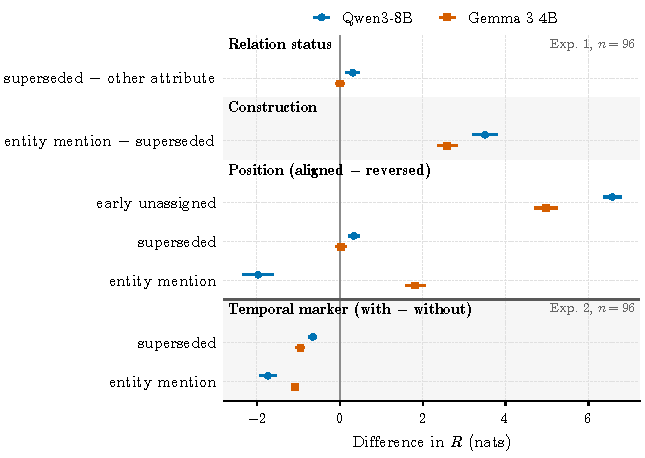
\includegraphics[width=0.68\linewidth]{figures/decomposition.pdf}
\end{center}
\caption{What changes query relevance. Every row is a difference in $R$ (nats) between two prompt variants, with 95\% history-bootstrap intervals. Relation status: superseded minus other attribute. Construction: entity mention minus superseded. Position: $R$ under aligned minus $R$ under reversed order, paired within history. Marker: $R$ with minus without \lit{Previously}, within each construction. Rows above the dark line come from Experiment 1 (96 histories); rows below it from Experiment 2 (96 histories, one entity pair and one attribute). Estimates are computed from the sealed analyses by \lit{scripts/fig\_decomposition.py}.}
\label{fig:decomposition}
\end{figure}

Table~\ref{tab:main} and Figure~\ref{fig:construction-order} give $R$ for every construction and order group. The live control shows the scale of a fully relevant edit: 32.598 nats in Qwen and 39.355 in Gemma. Superseded and other-attribute relevance are positive and similar in both order groups. Entity-mention relevance is the largest among the non-live constructions in both order groups. Unassigned relevance is near zero overall but large and of opposite sign in the two order groups.

\begin{table}[t]
\caption{Query relevance $R$ (nats) by construction and order group in Experiment 1, with 95\% history-bootstrap intervals over 96 histories. The live control has one assignment block, so it has no order split.}
\label{tab:main}
\begin{center}
\small
\begin{tabular}{@{}llrrr@{}}
\toprule
Model & Construction & Overall $R$ & Aligned $R$ & Reversed $R$ \\
\midrule
Qwen3-8B & Live & 32.598 [31.258, 33.967] & — & — \\
Qwen3-8B & Superseded & 1.974 [1.840, 2.109] & 2.144 [1.995, 2.301] & 1.804 [1.660, 1.947] \\
Qwen3-8B & Other attribute & 1.660 [1.488, 1.835] & 1.679 [1.527, 1.835] & 1.641 [1.422, 1.863] \\
Qwen3-8B & Entity mention & 5.478 [5.128, 5.825] & 4.493 [4.235, 4.770] & 6.463 [5.971, 6.940] \\
Qwen3-8B & Early unassigned & −0.037 [−0.203, 0.121] & 3.252 [3.046, 3.455] & −3.327 [−3.518, −3.150] \\
Qwen3-8B & Late unassigned & 0.001 [−0.208, 0.211] & 3.187 [2.948, 3.442] & −3.184 [−3.433, −2.945] \\
\midrule
Gemma 3 4B & Live & 39.355 [38.303, 40.415] & — & — \\
Gemma 3 4B & Superseded & 1.688 [1.568, 1.817] & 1.703 [1.574, 1.841] & 1.672 [1.529, 1.831] \\
Gemma 3 4B & Other attribute & 1.683 [1.541, 1.832] & 1.763 [1.598, 1.932] & 1.603 [1.453, 1.771] \\
Gemma 3 4B & Entity mention & 4.277 [4.029, 4.545] & 5.181 [4.884, 5.496] & 3.372 [3.131, 3.633] \\
Gemma 3 4B & Early unassigned & 0.113 [−0.023, 0.245] & 2.598 [2.395, 2.798] & −2.372 [−2.567, −2.178] \\
Gemma 3 4B & Late unassigned & 0.125 [−0.055, 0.305] & 3.445 [3.202, 3.696] & −3.194 [−3.447, −2.945] \\
\bottomrule
\end{tabular}
\end{center}
\end{table}

\begin{figure}[t]
\begin{center}
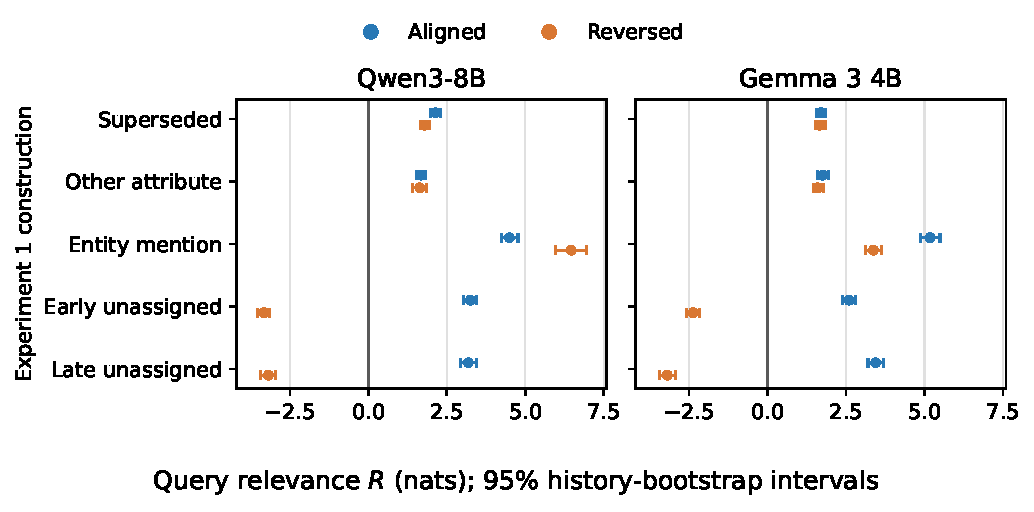
\includegraphics[width=0.98\linewidth]{figures/construction_by_order.pdf}
\end{center}
\caption{Query relevance $R$ (nats) for the five non-live constructions of Experiment 1, by order group and model. Points are means over 96 histories; intervals are 95\% history-bootstrap intervals. Live is omitted from the shared scale (Table~\ref{tab:main}). Paired order differences are in Table~\ref{tab:b-paired-r}.}
\label{fig:construction-order}
\end{figure}

These score changes coexist with correct rankings. In the superseded construction both models ranked the current value strictly first in all 1,536 baseline and all 1,536 edited prompts, with mean current-minus-earlier margins of 21.734 nats (Qwen) and 23.854 (Gemma). The edits changed source and donor scores that both had low absolute mass: Qwen's mean superseded source score fell from −22.271 to −23.881 while the donor score rose from −23.618 to −22.120 (Appendix~\ref{app:score-changes}). These changes do not imply that probability moves from one candidate to the other, or a matching change in generated answers.

\subsection{Relation status and construction}
\label{sec:relation}

Superseded minus other attribute is the study's closest estimate of what being an obsolete value of the queried attribute adds (Table~\ref{tab:frozen}; Section~\ref{sec:decomposition-logic} explains why it cannot separate the two properties involved). On average it adds 0.314 nats in Qwen, about a sixth of superseded relevance, and 0.004 in Gemma. The Qwen average masks heterogeneity: across target attributes it ranges from −0.570 for \lit{code} to 0.876 for \lit{color} (Table~\ref{tab:b-attr-other}); Gemma's attribute-specific intervals all include zero, which is not evidence of equivalence. Relation status is therefore small on average relative to construction, not uniformly negligible, and a follow-up shows that in Qwen the average combines two opposing effects (Section~\ref{sec:followups}).

Mentioning the earlier value in a note about the entity, without assigning it, produces more relevance than the superseded assignment in both models: superseded minus entity mention is −3.504 nats in Qwen and −2.589 in Gemma, and the sign holds for every target attribute (Table~\ref{tab:b-attr-entity}). The two constructions differ in predicate, syntax, name--value distance, and the presence of \lit{Previously}; Experiment 2 removes the marker difference (Section~\ref{sec:marker-results}) and a follow-up varies distance (Section~\ref{sec:followups}).

\begin{table}[t]
\caption{Superseded minus each control construction, $R_{\text{superseded}}-R_{\text{control}}$ (nats), with 95\% history-bootstrap intervals over 96 histories. Because early-unassigned $R$ is near zero after averaging over orders (Section~\ref{sec:order}), the last contrast is close to superseded $R$ itself. Order-stratified versions are in Table~\ref{tab:b-order}.}
\label{tab:frozen}
\begin{center}
\small
\begin{tabular}{@{}llrr@{}}
\toprule
Control & Isolates & Qwen3-8B & Gemma 3 4B \\
\midrule
Other attribute & relation status & 0.314 [0.147, 0.482] & 0.004 [−0.104, 0.118] \\
Entity mention & construction & −3.504 [−3.806, −3.198] & −2.589 [−2.829, −2.361] \\
Early unassigned & none: order-averaged control near zero & 2.011 [1.855, 2.170] & 1.575 [1.440, 1.719] \\
\bottomrule
\end{tabular}
\end{center}
\end{table}

These three contrasts were the test of our original hypothesis, which predicted that superseded relevance would exceed all three controls, each with a lower 95\% bound above zero, both overall and under reversed order. The prediction fails in both models, because the entity-mention contrast is negative overall and under reversed order (Table~\ref{tab:b-order}).

\subsection{Mention order}
\label{sec:order}

When no sentence links a value to an entity, the models link them by position. Under aligned order the first unassigned value sits in the same slot as the entity listed first in the current block, and an edit to it is more relevant to that entity's query; under reversed order the same value lines up with the other entity, and relevance turns negative (Table~\ref{tab:main}). The pattern holds for early and late unassigned mentions in both models, with paired order effects between 4.970 and 6.639 nats and positive in every one of the 96 histories (Table~\ref{tab:b-paired-r}). This is the behavior expected if values and entities are matched by ordinal position, consistent with the positional retrieval mechanism described by \citet{gurarieh2026mixing}; our data show the behavior, not the mechanism.

Explicit association does not remove order dependence, but it keeps relevance positive. Superseded relevance stays positive in both order groups (2.144 aligned and 1.804 reversed in Qwen; 1.703 and 1.672 in Gemma), with a small paired order effect. Entity-mention relevance also stays positive in both groups, but its paired order effect is large and model-specific: aligned order lowers it in Qwen (−1.969) and raises it in Gemma (+1.810). Averaging over orders hides the unassigned pattern entirely: overall unassigned relevance is near zero (−0.037 and 0.001 in Qwen; 0.113 and 0.125 in Gemma) not because the edit is ignored (an early unassigned edit shifts scores by 8.202 and 8.239 nats under the two queries in Qwen, and by 6.347 and 6.234 in Gemma) but because aligned and reversed effects cancel. The same cancellation makes superseded-minus-unassigned negative under aligned order and positive under reversed order (Figure~\ref{fig:order}, Appendix~\ref{app:exp1}).

\subsection{The explicit marker}
\label{sec:marker-results}

Experiment 2 adds or removes the prefix \lit{Previously,} with the rest of each prompt fixed (Table~\ref{tab:marker-templates}). Adding the marker lowers $R$ in both constructions and both models, with every within-construction interval below zero (Table~\ref{tab:marker}, Figure~\ref{fig:marker-effects}). In Qwen the reduction is larger for entity mentions: the marker-by-construction interaction is 1.082 [0.850, 1.308], positive in both order groups. In Gemma the two reductions are similar and the interaction, 0.125 [−0.012, 0.265], is not resolved; its order groups point in opposite directions. An earlier 24-history run of the same design gave the same pattern (Appendix~\ref{app:marker}). Relevance stays positive with the marker in every construction and order group, so the marker lowers the earlier value's influence without removing it. A lower score contrast is not evidence of active suppression.

Without the marker, entity-mention relevance still exceeds superseded relevance: by 3.059 [2.758, 3.370] nats in Qwen and 0.908 [0.783, 1.034] in Gemma, paired within history. The gap depends on order, however. In Gemma's reversed-order cell the difference is not resolved (entity minus superseded −0.175 [−0.357, 0.011]), and the marker leaves Gemma's gap almost unchanged (0.782 [0.673, 0.894] with the marker). An exploratory Phi-4-mini run on the earlier 24-history dataset showed yet another pattern, with the marker lowering superseded relevance (−1.355 [−1.561, −1.138]) but not entity-mention relevance (0.145 [−0.018, 0.310]; Appendix~\ref{app:marker}).

\begin{table}[t]
\caption{The four historical-line templates of Experiment 2, shown for Nora. Each prompt has two such lines, one per entity, followed by the current-state block and query of Experiment 1.}
\label{tab:marker-templates}
\begin{center}
\small
\begin{tabular}{@{}l>{\raggedright\arraybackslash}p{0.33\linewidth}>{\raggedright\arraybackslash}p{0.40\linewidth}@{}}
\toprule
Construction & Marker absent & Marker present \\
\midrule
Superseded & \lit{Nora's badge was amber.} & \lit{Previously, Nora's badge was amber.} \\
Entity mention & \lit{Nora mentioned amber in an unrelated note.} & \lit{Previously, Nora mentioned amber in an unrelated note.} \\
\bottomrule
\end{tabular}
\end{center}
\end{table}

\begin{table}[t]
\caption{Marker effects, $R_{\text{present}}-R_{\text{absent}}$, and the marker-by-construction interaction (superseded minus entity-mention marker effect) in Experiment 2, in nats, with 95\% history-bootstrap intervals over 96 histories. The underlying $R$ values, their source/donor components, and the earlier 24-history run are in Appendix~\ref{app:marker}.}
\label{tab:marker}
\begin{center}
\small
\begin{tabular}{@{}llrrr@{}}
\toprule
Model & Order & Superseded & Entity mention & Interaction \\
\midrule
Qwen3-8B & All & −0.652 [−0.748, −0.560] & −1.734 [−1.934, −1.536] & 1.082 [0.850, 1.308] \\
Qwen3-8B & Aligned & −0.366 [−0.484, −0.243] & −1.000 [−1.164, −0.834] & 0.635 [0.427, 0.841] \\
Qwen3-8B & Reversed & −0.938 [−1.071, −0.804] & −2.469 [−2.746, −2.189] & 1.530 [1.208, 1.847] \\
\midrule
Gemma 3 4B & All & −0.950 [−1.062, −0.841] & −1.075 [−1.166, −0.986] & 0.125 [−0.012, 0.265] \\
Gemma 3 4B & Aligned & −0.963 [−1.100, −0.834] & −1.445 [−1.566, −1.326] & 0.482 [0.307, 0.655] \\
Gemma 3 4B & Reversed & −0.937 [−1.112, −0.767] & −0.705 [−0.833, −0.580] & −0.232 [−0.436, −0.027] \\
\bottomrule
\end{tabular}
\end{center}
\end{table}

\begin{figure}[t]
\begin{center}
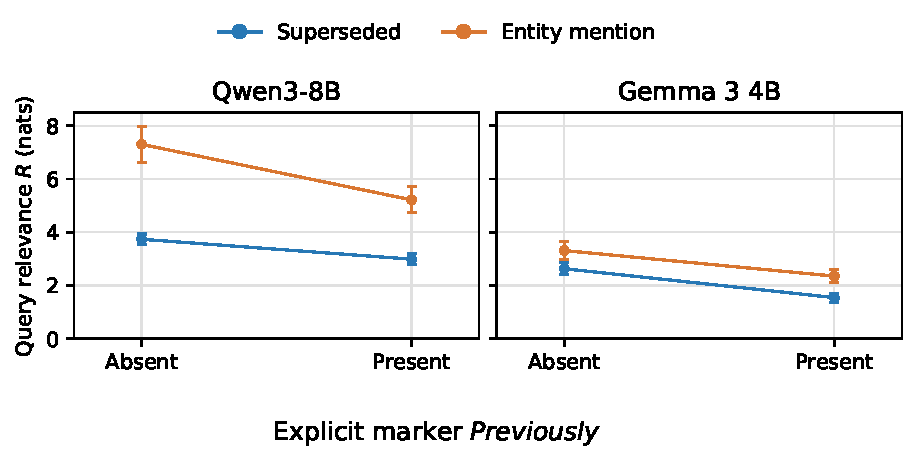
\includegraphics[width=0.78\linewidth]{figures/marker_by_construction.pdf}
\end{center}
\caption{Query relevance in Experiment 2 by marker and construction, averaged over orders. Points are means over 96 histories; intervals are marginal 95\% history-bootstrap intervals. Paired marker effects and the interaction, rather than overlap of marginal intervals, are in Table~\ref{tab:marker}.}
\label{fig:marker-effects}
\end{figure}

\subsection{Follow-up experiments}
\label{sec:followups}

\paragraph{Relation status splits into two opposing effects in Qwen.} With prompt length and layout matched, having been the queried attribute raised relevance (superseded minus updated other attribute: 0.740 [0.661, 0.818] nats in Qwen, 0.148 [0.038, 0.261] in Gemma), while being contradicted by an update lowered it in Qwen (updated minus static other attribute: −0.289 [−0.363, −0.215]) but not detectably in Gemma (−0.028 [−0.137, 0.076]; Table~\ref{tab:update}). In Qwen the two effects partly cancel, which is why the joint contrast of Experiment 1 was small; the recorded prediction of the discount account holds for Qwen and is unresolved for Gemma.

\begin{table}[t]
\caption{Updated-other-attribute follow-up: $R$ (nats) by construction and the two contrasts it separates, with 95\% history-bootstrap intervals over 96 histories. All three constructions share a six-line layout.}
\label{tab:update}
\begin{center}
\small
\begin{tabular}{@{}lrr@{}}
\toprule
 & Qwen3-8B & Gemma 3 4B \\
\midrule
Superseded & 1.368 [1.282, 1.457] & 0.817 [0.713, 0.928] \\
Other attribute, updated & 0.628 [0.555, 0.700] & 0.669 [0.568, 0.770] \\
Other attribute, not updated & 0.917 [0.835, 1.003] & 0.697 [0.602, 0.802] \\
\midrule
Queried attribute (superseded $-$ updated) & 0.740 [0.661, 0.818] & 0.148 [0.038, 0.261] \\
Update (updated $-$ not updated) & −0.289 [−0.363, −0.215] & −0.028 [−0.137, 0.076] \\
Superseded $-$ not updated & 0.451 [0.376, 0.525] & 0.120 [0.027, 0.209] \\
\bottomrule
\end{tabular}
\end{center}
\end{table}

\paragraph{Name--value distance does not explain the construction gap.} Moving the name next to the value raised superseded relevance in both models (near minus far: 0.500 [0.400, 0.599] in Qwen, 0.393 [0.288, 0.496] in Gemma) but did not raise entity-mention relevance: the near-minus-far difference was −0.370 [−0.498, −0.249] in Qwen and −0.027 [−0.110, 0.058] in Gemma (Table~\ref{tab:distance}). The recorded prediction, near above far in both constructions, therefore fails in both models; in Qwen's entity-mention construction the effect goes the other way. At matched near distance (one token between name and value in both constructions), entity mentions remain more influential than superseded assignments, by 1.293 [1.019, 1.571] nats in Qwen and 0.367 [0.234, 0.514] in Gemma, smaller than the far-condition gaps of 2.163 and 0.788. Proximity raises superseded relevance and so closes part of the gap, but not most of it in Qwen and not all of it in either model.

\begin{table}[t]
\caption{Name--value distance follow-up: $R$ (nats) by construction and distance, near-minus-far differences, and the entity-minus-superseded gap at each distance, with 95\% history-bootstrap intervals over 96 histories. Measured name--value gaps: one token in both near conditions; three (Qwen) or four (Gemma) tokens for superseded far; seven for entity-mention far.}
\label{tab:distance}
\begin{center}
\small
\begin{tabular}{@{}lrr@{}}
\toprule
 & Qwen3-8B & Gemma 3 4B \\
\midrule
Superseded, near & 2.685 [2.516, 2.861] & 2.005 [1.858, 2.135] \\
Superseded, far & 2.184 [2.030, 2.335] & 1.612 [1.492, 1.735] \\
Entity mention, near & 3.977 [3.684, 4.264] & 2.372 [2.245, 2.505] \\
Entity mention, far & 4.347 [4.043, 4.662] & 2.399 [2.261, 2.545] \\
\midrule
Superseded, near $-$ far & 0.500 [0.400, 0.599] & 0.393 [0.288, 0.496] \\
Entity mention, near $-$ far & −0.370 [−0.498, −0.249] & −0.027 [−0.110, 0.058] \\
\midrule
Entity $-$ superseded, near & 1.293 [1.019, 1.571] & 0.367 [0.234, 0.514] \\
Entity $-$ superseded, far & 2.163 [1.866, 2.459] & 0.788 [0.657, 0.922] \\
\bottomrule
\end{tabular}
\end{center}
\end{table}

Read across experiments, the construction gap shrinks as the two constructions are made more alike (Table~\ref{tab:gap}). In Experiment 1 only the superseded line carries \lit{Previously} and its value sits three or four tokens after the name, against one token in the entity-mention line; there the gap is 3.504 nats in Qwen and 2.589 in Gemma. With the marker on both lines it is 1.976 and 0.782 in Experiment 2, and with the marker on both lines and a one-token name--value distance in both it is 1.293 and 0.367 in the distance follow-up. The rows come from different stimulus sets (Experiment 2 uses one entity pair and one attribute), so they are matched comparisons rather than an additive decomposition. What remains at matched marker and distance, about 1.3 nats in Qwen and 0.4 in Gemma, is the part that predicate and framing would have to explain.

\begin{table}[t]
\caption{Entity-mention minus superseded relevance (nats) under increasingly matched conditions, with 95\% history-bootstrap intervals. ``Marker'' gives which construction carries \lit{Previously}; ``Gap'' gives the measured tokens between name and value (entity mention vs.\ superseded). Experiment 2 uses one entity pair and one attribute; the other rows use Experiment 1's allocation.}
\label{tab:gap}
\begin{center}
\small
\begin{tabular}{@{}llllrr@{}}
\toprule
Source & Marker & Gap & Histories & Qwen3-8B & Gemma 3 4B \\
\midrule
Experiment 1 & superseded only & 1 vs.\ 3--4 & 96 & 3.504 [3.198, 3.806] & 2.589 [2.361, 2.829] \\
Experiment 2 & neither & 1 vs.\ 3--4 & 96 & 3.059 [2.758, 3.370] & 0.908 [0.783, 1.034] \\
Experiment 2 & both & 1 vs.\ 3--4 & 96 & 1.976 [1.795, 2.169] & 0.782 [0.673, 0.894] \\
Distance follow-up, far & both & 7 vs.\ 3--4 & 96 & 2.163 [1.866, 2.459] & 0.788 [0.657, 0.922] \\
Distance follow-up, near & both & 1 vs.\ 1 & 96 & 1.293 [1.019, 1.571] & 0.367 [0.234, 0.514] \\
\bottomrule
\end{tabular}
\end{center}
\end{table}

\paragraph{More updates, more sensitivity in Qwen, while answers stay correct.} Both models answered every development prompt correctly at chain depths 3, 4, and 5 (384 generated answers per depth and model), so no depth fell in the 70--95\% window and, by the recorded rule, no generation confirmation was run. The candidate scores told a different story. On 96 histories per depth, Qwen's $R$ for the edited superseded value rose from 7.353 [6.972, 7.725] nats at depth 3 to 10.762 [10.303, 11.220] at depth 4 and 11.835 [11.424, 12.286] at depth 5; the depth-5-minus-depth-3 difference of 4.482 [3.915, 5.047] meets the recorded criterion. Gemma's $R$ stayed between 3.450 and 3.708 (depth 5 minus depth 3: 0.258 [−0.063, 0.557]). In Qwen, then, each additional update makes the scores more sensitive to the most recent superseded value even though no answer names it, a score-level counterpart of the interference that \citet{wang2025unable} observe in answers when updates accumulate (Appendix~\ref{app:followups}). Neither the chains nor the earlier distractor study (Appendix~\ref{app:harder}) lowered accuracy enough to test generated answers.

\paragraph{Below ceiling, generated answers follow the same pattern (exploratory).} OLMo-2's answers were correct for 2,950 of 3,072 superseded prompts but only 1,846 of 3,072 entity-mention prompts and 1,528 and 2,131 of the early- and late-unassigned prompts (Table~\ref{tab:olmo}). Its errors follow the pattern of the screened models' scores. Editing a value mentioned with the queried entity moved answers to the donor query-specifically (donor following 0.155 [0.124, 0.190]). Never-assigned values were named in about a tenth of answers and pulled them toward the entity in the matching position: early-unassigned donor following was 0.161 [0.122, 0.203] under aligned order and −0.164 [−0.214, −0.120] under reversed order, cancelling when orders are pooled. Superseded and other-attribute values almost never surfaced (0.9\% and 0.1\% of baseline answers to the edited entity's query named its earlier value), although the superseded edit still moved answers by a small, query-specific amount (0.008 [0.003, 0.014]). Where answers are not at ceiling, then, the earlier values that change scores are also the ones that change answers.

\begin{table}[t]
\caption{Exploratory generated-answer study in OLMo-2-7B-Instruct (outside the screened population) on the Experiment 1 confirmation set. Accuracy counts all 3,072 prompts per construction; donor following is the share of edited prompts answered with the donor under the edited entity's query minus under the other entity's query, with 95\% history-bootstrap intervals over 96 histories.}
\label{tab:olmo}
\begin{center}
\small
\begin{tabular}{@{}lrrrr@{}}
\toprule
Construction & Accuracy & Donor following & Aligned & Reversed \\
\midrule
Live & 2,970/3,072 & 0.948 [0.924, 0.969] & 0.948 & 0.948 \\
Superseded & 2,950/3,072 & 0.008 [0.003, 0.014] & 0.016 & 0.000 \\
Other attribute & 2,990/3,072 & 0.001 [0.000, 0.004] & 0.000 & 0.003 \\
Entity mention & 1,846/3,072 & 0.155 [0.124, 0.190] & 0.185 & 0.125 \\
Early unassigned & 1,528/3,072 & −0.001 [−0.022, 0.020] & 0.161 & −0.164 \\
Late unassigned & 2,131/3,072 & 0.005 [−0.022, 0.031] & 0.148 & −0.138 \\
\bottomrule
\end{tabular}
\end{center}
\end{table}

\paragraph{Additional models.} OLMo-2-7B-Instruct failed the competence screen, ranking the current value first on 426--452 of 576 prompts in the entity-mention and unassigned constructions (Appendix~\ref{app:followups}); by the protocol it is not part of the screened analysis. Qwen3-14B could not be loaded with int8 weights on the 16 GB GPU used for every other run. Phi-4-mini again failed the screen in entity mention (561/576); scored descriptively on the confirmation set, it resembled the screened models in construction and order, with entity-mention relevance above superseded relevance by 1.872 [1.664, 2.091] nats and order-averaged early-unassigned relevance near zero (0.027 [−0.069, 0.130]). Unlike them, its superseded relevance was slightly below other-attribute relevance (−0.152 [−0.266, −0.040]).

\section{Discussion}
\label{sec:discussion}

Read together, the comparisons say that a model's sensitivity to an earlier value tracks how that value is attached to an entity in the text, not what the value used to mean. A value that was the queried attribute and has since been updated, and a value that was some other attribute of the same entity and was never updated, differ by at most a third of a nat, although only the first is contradicted by the current state. A value placed in a sentence with the entity, even a note described as unrelated, is several nats more influential than either. A value attached to no one is credited to whichever entity shares its position. The word \lit{Previously} turns the influence down but not off. For the problem that motivated this work---whether models retain obsolete assignments---the answer from these scores is that the residual sensitivity we measure is not specific to obsolescence: the same sensitivity arises for values that were never assigned to the queried attribute at all.

The positional result connects our short prompts to findings in much longer ones. \citet{liu2024lost} and \citet{yang2026conflicts} report that where evidence appears changes how models use it, and \citet{gurarieh2026mixing} describe a positional mechanism for retrieving bound entities. Six-line contexts already show order deciding which entity an unattached value is credited to. A practical consequence for evaluation is that averaging over mention orders can produce null effects that conceal large opposing ones, as the near-zero overall relevance of unassigned values does here.

One gap remains open. Entity-mention relevance exceeds superseded relevance in Experiment 1, where only the superseded construction carries \lit{Previously}, and the gap persists in Experiment 2 when neither carries it: without the marker, $R$ is 7.304 [6.629, 7.966] for entity mention and 3.738 [3.536, 3.934] for superseded in Qwen, and 3.313 [2.975, 3.669] and 2.631 [2.409, 2.863] in Gemma. The two constructions still differ in predicate and word order. One property they differ in is the distance between the entity name and the value: in \lit{Nora mentioned amber}, the value follows the name after one word, while in \lit{Nora’s badge was amber} it follows the attribute and the copula. Given that relative position governs unattached values, we hypothesize that name--value proximity explains the construction gap. This predicts that moving the value closer to the name raises relevance within a construction, and that the gap shrinks at matched distance. [TODO: run P1.1 name--value distance test.]

The measure has a deliberately narrow scope. Scores are bounded masses of fixed answer prefixes, not probabilities of generated answers, and the models answer at ceiling: the current value is top-ranked in every superseded trial. At ceiling, the earlier value does not surface in generated answers: in a variant of Experiment 1 with two to six added distractor entities, neither model answered any of 1,152 superseded prompts with the earlier value (Appendix~\ref{app:harder}). Whether the score shifts change generated answers below ceiling is untested. Adding distractors did not lower accuracy enough to test it---Qwen stayed above 99.6\% at every level, which triggered that study's prespecified stopping rule. [TODO: run P1.3 harder-task redesign.] The experiments use two models, English prompts with two target entities, an eight-value vocabulary, and one set of sentence templates per experiment; generalization beyond these is untested.

\section{Conclusion}
\label{sec:conclusion}

In these two models and prompt sets, replacing an earlier value causally changes bounded candidate scores, and the query-specific contrast varies across the tested mention constructions and orders. The findings do not identify independent contributions from entity association, relation status, position, and temporal meaning, nor an internal obsolete-binding mechanism. Unassigned-value relevance reverses with mention order in both models, while entity-mention order effects differ in direction between models. The average superseded-minus-other-attribute contrast is modest relative to the entity-mention contrast, but Qwen's attribute-specific estimates vary in sign. Thus, this score measure is sensitive to prompt construction and order and does not uniquely diagnose an obsolete assignment. Further tests across templates, attributes, and models are needed before generalizing beyond these stimuli.


\bibliography{references}
\bibliographystyle{tmlr}

\appendix
% Number appendix tables per appendix (Table B1, B2, ...).
\counterwithin{table}{section}
\renewcommand{\thetable}{\thesection\arabic{table}}

\section{The preliminary comparison and a derived-code task}
\label{app:prelim}

\subsection{Preliminary comparison}
\label{sec:prelim}

Experiment 1 was motivated by an earlier, simpler comparison with different sentence templates. It contrasted superseded assignments with a single control in which the two earlier values were mentioned as unassigned values, averaging the two mention orders. Superseded relevance exceeded this control in all three models that passed that comparison's competence screen: by 3.50 nats (95\% CI [3.20, 3.80]) in Qwen3-8B, 1.76 [1.51, 2.03] in Gemma 3 4B, and 5.53 [5.27, 5.79] in Phi-4-mini. Read alone, this looks like evidence that superseded assignments retain query-specific influence. But the control matched neither the entity association nor the relative position of the superseded mentions, so the comparison could not say which property produced the difference. Experiment 1 adds controls for each.

The preliminary comparison used different templates from Experiments 1 and 2. A superseded prompt for the Nora/Liam example read:

\begin{prompt}
The badge assigned to Nora was amber.
The badge assigned to Liam was coral.
Later, Nora’s badge was changed to jade.
Later, Liam’s badge was changed to pearl.
What is Nora’s current badge?
Respond with only the value, with no explanation.
\end{prompt}

The control stated the current assignments and mentioned \lit{amber} and \lit{coral} as unassigned badge values, in both mention orders; the primary contrast averaged the two orders within each history. A live control edited the current assignment. Scoring, $E$, and $R$ were defined as in Section~\ref{sec:task}. Each history contributed 40 scored prompts, giving 3,840 prompts and 1,920 matched edit pairs over 96 confirmation histories per model, with the same history-level bootstrap. Four models were screened with the same 99\% rule. Qwen3-8B, Gemma 3 4B, and Phi-4-mini passed; Mistral-7B-Instruct-v0.3 scored 281/288 on the unassigned control and was not run.

\subsection{Derived-code task}
\label{app:derived-code}

To ask whether sensitivity to an earlier value reaches a computation that uses it, we mapped values to shuffled opaque codes and asked which code corresponded to an entity's current badge. The codebook stayed fixed across baseline and edit; editing an earlier badge value changed which code it mapped to, not the codebook or the current assignment. We scored all 16 full code sequences by their unnormalized log probability. Only Qwen passed this task's screen (48/48); its threshold, 47/48 (97.9\%), was specific to this task and recorded before scoring. Gemma scored 45/48 and Phi 33/48. For Qwen, query relevance was 5.544 nats (95\% CI [5.159, 5.941]) for an edit to the earlier value and 12.836 [12.418, 13.257] for an edit to the current value, both positive in all 96 histories. Qwen's candidate ranking is below ceiling here: with the earlier value edited, the current code ranked first in 360/384 baseline and 364/384 edited prompts; 9 pairs changed from incorrect to correct and 5 from correct to incorrect. Changes in the current code's log probability (0.108 [−0.050, 0.264]) and in the candidate margin (0.103 [−0.118, 0.325]) had intervals spanning zero. This task lacks the entity-mention and order controls of Experiment 1 and collected no generated answers, so it shows score sensitivity in a derived computation, below ceiling in candidate ranking, without saying which property of the earlier mention produces it or whether generated answers change.

\FloatBarrier

\section{Additional results for Experiment 1}
\label{app:exp1}

All intervals in this appendix are 95\% history-bootstrap intervals (Section~\ref{sec:inference}).

\subsection{Query relevance by construction and order}

Table~\ref{tab:main} and Figure~\ref{fig:construction-order} give $R$ for every construction and order group, and Table~\ref{tab:frozen} the three superseded-minus-control contrasts that tested the original hypothesis. Superseded and other-attribute relevance are positive and similar in both order groups; entity-mention relevance is the largest among the non-live constructions; unassigned relevance is near zero overall but large and of opposite sign in the two order groups.

\begin{table}[t]
\caption{Query relevance $R$ (nats) by construction and order group in Experiment 1, with 95\% history-bootstrap intervals over 96 histories. The live control has one assignment block, so it has no order split.}
\label{tab:main}
\begin{center}
\small
\begin{tabular}{@{}llrrr@{}}
\toprule
Model & Construction & Overall $R$ & Aligned $R$ & Reversed $R$ \\
\midrule
Qwen3-8B & Live & 32.598 [31.258, 33.967] & — & — \\
Qwen3-8B & Superseded & 1.974 [1.840, 2.109] & 2.144 [1.995, 2.301] & 1.804 [1.660, 1.947] \\
Qwen3-8B & Other attribute & 1.660 [1.488, 1.835] & 1.679 [1.527, 1.835] & 1.641 [1.422, 1.863] \\
Qwen3-8B & Entity mention & 5.478 [5.128, 5.825] & 4.493 [4.235, 4.770] & 6.463 [5.971, 6.940] \\
Qwen3-8B & Early unassigned & −0.037 [−0.203, 0.121] & 3.252 [3.046, 3.455] & −3.327 [−3.518, −3.150] \\
Qwen3-8B & Late unassigned & 0.001 [−0.208, 0.211] & 3.187 [2.948, 3.442] & −3.184 [−3.433, −2.945] \\
\midrule
Gemma 3 4B & Live & 39.355 [38.303, 40.415] & — & — \\
Gemma 3 4B & Superseded & 1.688 [1.568, 1.817] & 1.703 [1.574, 1.841] & 1.672 [1.529, 1.831] \\
Gemma 3 4B & Other attribute & 1.683 [1.541, 1.832] & 1.763 [1.598, 1.932] & 1.603 [1.453, 1.771] \\
Gemma 3 4B & Entity mention & 4.277 [4.029, 4.545] & 5.181 [4.884, 5.496] & 3.372 [3.131, 3.633] \\
Gemma 3 4B & Early unassigned & 0.113 [−0.023, 0.245] & 2.598 [2.395, 2.798] & −2.372 [−2.567, −2.178] \\
Gemma 3 4B & Late unassigned & 0.125 [−0.055, 0.305] & 3.445 [3.202, 3.696] & −3.194 [−3.447, −2.945] \\
\bottomrule
\end{tabular}
\end{center}
\end{table}

\begin{figure}[t]
\begin{center}
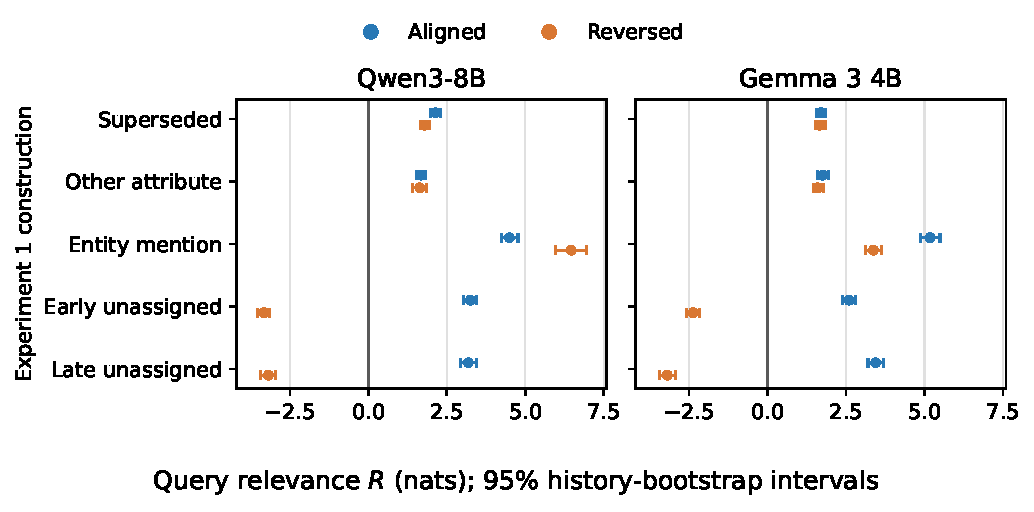
\includegraphics[width=0.98\linewidth]{figures/construction_by_order.pdf}
\end{center}
\caption{Query relevance $R$ (nats) for the five non-live constructions of Experiment 1, by order group and model. Points are means over 96 histories; intervals are 95\% history-bootstrap intervals. Live is omitted from the shared scale (Table~\ref{tab:main}). Paired order differences are in Table~\ref{tab:b-paired-r}.}
\label{fig:construction-order}
\end{figure}

\begin{table}[t]
\caption{Superseded minus each control construction, $R_{\text{superseded}}-R_{\text{control}}$ (nats), with 95\% history-bootstrap intervals over 96 histories. Because early-unassigned $R$ is near zero after averaging over orders (Section~\ref{sec:order}), the last contrast is close to superseded $R$ itself. Order-stratified versions are in Table~\ref{tab:b-order}.}
\label{tab:frozen}
\begin{center}
\small
\begin{tabular}{@{}llrr@{}}
\toprule
Control & Isolates & Qwen3-8B & Gemma 3 4B \\
\midrule
Other attribute & relation status & 0.314 [0.147, 0.482] & 0.004 [−0.104, 0.118] \\
Entity mention & construction & −3.504 [−3.806, −3.198] & −2.589 [−2.829, −2.361] \\
Early unassigned & none: order-averaged control near zero & 2.011 [1.855, 2.170] & 1.575 [1.440, 1.719] \\
\bottomrule
\end{tabular}
\end{center}
\end{table}

\subsection{Order groups}

Table~\ref{tab:b-paired-r} gives the paired order effect on $R$ itself for each construction, Table~\ref{tab:b-order} each superseded-minus-control contrast by order group, and Table~\ref{tab:b-paired} the paired difference between the aligned and reversed contrasts. Paired differences are computed within history. The live control has one assignment block and no order split.

\begin{figure}[h]
\begin{center}
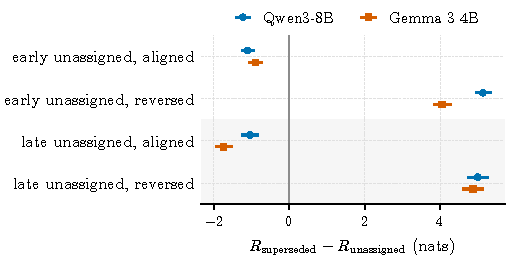
\includegraphics[width=0.58\linewidth]{figures/order_stratified_contrasts.pdf}
\end{center}
\caption{Superseded-minus-unassigned relevance contrasts by order group, in nats, with 95\% history-bootstrap intervals. The contrasts are negative under aligned order and positive under reversed order in both models. The comparison depends on both construction and order; it does not imply that construction is irrelevant.}
\label{fig:order}
\end{figure}

\begin{table}[h]
\caption{Paired order effect on query relevance, $R_{\text{aligned}}-R_{\text{reversed}}$ (nats), computed within history, with the fraction of the 96 histories in which it is positive.}
\label{tab:b-paired-r}
\begin{center}
\small
\begin{tabular}{@{}lrr@{}}
\toprule
Construction & Qwen3-8B & Gemma 3 4B \\
\midrule
Superseded & 0.340 [0.218, 0.470]; 0.688 & 0.032 [−0.101, 0.168]; 0.531 \\
Entity mention & −1.969 [−2.344, −1.604]; 0.135 & 1.810 [1.580, 2.058]; 0.958 \\
Early unassigned & 6.578 [6.356, 6.789]; 1.000 & 4.970 [4.700, 5.257]; 1.000 \\
Late unassigned & 6.371 [6.113, 6.646]; 1.000 & 6.639 [6.308, 6.967]; 1.000 \\
\bottomrule
\end{tabular}
\end{center}
\end{table}

\begin{table}[h]
\caption{Superseded minus control, $R_{\text{superseded}}-R_{\text{control}}$ (nats), by order group. Overall values are in Table~\ref{tab:frozen}.}
\label{tab:b-order}
\begin{center}
\small
\begin{tabular}{@{}llrr@{}}
\toprule
Control & Order & Qwen3-8B & Gemma 3 4B \\
\midrule
Other attribute & Aligned & 0.465 [0.295, 0.649] & −0.060 [−0.215, 0.099] \\
Other attribute & Reversed & 0.162 [−0.049, 0.367] & 0.069 [−0.080, 0.213] \\
Entity mention & Aligned & −2.350 [−2.572, −2.125] & −3.478 [−3.769, −3.197] \\
Entity mention & Reversed & −4.659 [−5.119, −4.207] & −1.700 [−1.946, −1.465] \\
Early unassigned & Aligned & −1.108 [−1.281, −0.925] & −0.895 [−1.084, −0.719] \\
Early unassigned & Reversed & 5.130 [4.920, 5.348] & 4.044 [3.810, 4.292] \\
Late unassigned & Overall & 1.973 [1.762, 2.183] & 1.562 [1.390, 1.742] \\
Late unassigned & Aligned & −1.043 [−1.281, −0.810] & −1.741 [−1.968, −1.505] \\
Late unassigned & Reversed & 4.988 [4.724, 5.266] & 4.866 [4.592, 5.155] \\
\bottomrule
\end{tabular}
\end{center}
\end{table}

\begin{table}[h]
\caption{Paired aligned-minus-reversed differences in the superseded-minus-control contrast (nats).}
\label{tab:b-paired}
\begin{center}
\small
\begin{tabular}{@{}lrr@{}}
\toprule
Control & Qwen3-8B & Gemma 3 4B \\
\midrule
Other attribute & 0.302 [0.103, 0.509] & −0.128 [−0.323, 0.081] \\
Entity mention & 2.309 [1.933, 2.707] & −1.778 [−2.049, −1.519] \\
Early unassigned & −6.238 [−6.481, −5.983] & −4.939 [−5.275, −4.620] \\
Late unassigned & −6.031 [−6.307, −5.754] & −6.607 [−6.951, −6.243] \\
\bottomrule
\end{tabular}
\end{center}
\end{table}

\subsection{Accuracy and correctly answered histories}

Table~\ref{tab:b-accuracy} gives strict rank-one accuracy over all 3,072 scored prompts per construction in the main experiment, counting baseline and edited prompts and repeated renderings of identical prompts.

\begin{table}[h]
\caption{Strict rank-one candidate accuracy in Experiment 1, per construction.}
\label{tab:b-accuracy}
\begin{center}
\small
\begin{tabular}{@{}lrr@{}}
\toprule
Construction & Qwen3-8B & Gemma 3 4B \\
\midrule
Live & 3,064/3,072 (99.7396\%) & 3,072/3,072 (100\%) \\
Superseded & 3,072/3,072 (100\%) & 3,072/3,072 (100\%) \\
Other attribute & 3,072/3,072 (100\%) & 3,072/3,072 (100\%) \\
Entity mention & 3,072/3,072 (100\%) & 3,072/3,072 (100\%) \\
Early unassigned & 3,072/3,072 (100\%) & 3,071/3,072 (99.9674\%) \\
Late unassigned & 3,069/3,072 (99.9023\%) & 3,072/3,072 (100\%) \\
\bottomrule
\end{tabular}
\end{center}
\end{table}

Restricting the analysis to histories in which every prompt was answered correctly retains 91/96 Qwen and 95/96 Gemma histories and leaves the contrasts essentially unchanged (Table~\ref{tab:b-selected}).

\begin{table}[h]
\caption{Superseded minus control (nats) among histories with every prompt ranked correctly.}
\label{tab:b-selected}
\begin{center}
\small
\begin{tabular}{@{}lrr@{}}
\toprule
Control & Qwen3-8B (91 histories) & Gemma 3 4B (95 histories) \\
\midrule
Other attribute & 0.371 [0.201, 0.532] & 0.004 [−0.106, 0.119] \\
Entity mention & −3.445 [−3.750, −3.141] & −2.591 [−2.827, −2.354] \\
Early unassigned & 2.015 [1.861, 2.176] & 1.576 [1.433, 1.714] \\
\bottomrule
\end{tabular}
\end{center}
\end{table}

\subsection{Source and donor score changes}
\label{app:score-changes}

Table~\ref{tab:b-abs-mass} gives the absolute log masses of the source, donor, and current candidates before and after the edit, and Table~\ref{tab:b-score-changes} the mean changes. The source and donor masses are low in every construction except live, so a change of several nats between them does not imply that probability moves from one to the other.

\begin{table}[h]
\caption{Absolute candidate log masses $S$ (nats) in Experiment 1: mean over prompts, with the first and third quartiles below. Source is the edited earlier value, donor its replacement, current the correct answer; 1,536 baseline and 1,536 edited prompts per construction and model. In the live construction the source is the current value of the edited entity, so its mass is high when that entity is queried.}
\label{tab:b-abs-mass}
\begin{center}
\resizebox{\linewidth}{!}{%
\begin{tabular}{@{}lrrrrrr@{}}
\toprule
 & \multicolumn{2}{c}{Source} & \multicolumn{2}{c}{Donor} & \multicolumn{2}{c}{Current} \\
\cmidrule(lr){2-3}\cmidrule(lr){4-5}\cmidrule(l){6-7}
Construction & Baseline & Edited & Baseline & Edited & Baseline & Edited \\
\midrule
\multicolumn{7}{@{}l}{\emph{Qwen3-8B}} \\
Live & \shortstack[r]{−8.027\\[-1pt]\scriptsize(−16.124, −0.000)} & \shortstack[r]{−23.650\\[-1pt]\scriptsize(−26.373, −20.584)} & \shortstack[r]{−24.086\\[-1pt]\scriptsize(−26.850, −20.941)} & \shortstack[r]{−8.132\\[-1pt]\scriptsize(−16.394, −0.000)} & \shortstack[r]{−0.004\\[-1pt]\scriptsize(−0.000, −0.000)} & \shortstack[r]{−0.012\\[-1pt]\scriptsize(−0.000, −0.000)} \\
Superseded & \shortstack[r]{−22.271\\[-1pt]\scriptsize(−24.703, −19.578)} & \shortstack[r]{−23.881\\[-1pt]\scriptsize(−26.425, −21.172)} & \shortstack[r]{−23.618\\[-1pt]\scriptsize(−25.922, −20.888)} & \shortstack[r]{−22.120\\[-1pt]\scriptsize(−24.476, −19.328)} & \shortstack[r]{−0.000\\[-1pt]\scriptsize(−0.000, −0.000)} & \shortstack[r]{−0.000\\[-1pt]\scriptsize(−0.000, −0.000)} \\
Other attribute & \shortstack[r]{−21.048\\[-1pt]\scriptsize(−23.317, −18.476)} & \shortstack[r]{−22.396\\[-1pt]\scriptsize(−24.662, −19.810)} & \shortstack[r]{−22.234\\[-1pt]\scriptsize(−24.235, −19.717)} & \shortstack[r]{−20.903\\[-1pt]\scriptsize(−22.978, −18.297)} & \shortstack[r]{−0.000\\[-1pt]\scriptsize(−0.000, −0.000)} & \shortstack[r]{−0.000\\[-1pt]\scriptsize(−0.000, −0.000)} \\
Entity mention & \shortstack[r]{−19.836\\[-1pt]\scriptsize(−23.242, −16.699)} & \shortstack[r]{−23.668\\[-1pt]\scriptsize(−26.370, −20.562)} & \shortstack[r]{−23.452\\[-1pt]\scriptsize(−26.000, −20.390)} & \shortstack[r]{−19.868\\[-1pt]\scriptsize(−23.344, −16.464)} & \shortstack[r]{−0.001\\[-1pt]\scriptsize(−0.000, −0.000)} & \shortstack[r]{−0.001\\[-1pt]\scriptsize(−0.000, −0.000)} \\
Early unassigned & \shortstack[r]{−16.488\\[-1pt]\scriptsize(−18.781, −14.193)} & \shortstack[r]{−20.697\\[-1pt]\scriptsize(−22.808, −18.257)} & \shortstack[r]{−20.497\\[-1pt]\scriptsize(−22.524, −18.016)} & \shortstack[r]{−16.485\\[-1pt]\scriptsize(−18.609, −13.922)} & \shortstack[r]{−0.000\\[-1pt]\scriptsize(−0.000, −0.000)} & \shortstack[r]{−0.000\\[-1pt]\scriptsize(−0.000, −0.000)} \\
Late unassigned & \shortstack[r]{−17.218\\[-1pt]\scriptsize(−19.385, −14.906)} & \shortstack[r]{−23.119\\[-1pt]\scriptsize(−25.287, −20.589)} & \shortstack[r]{−22.899\\[-1pt]\scriptsize(−25.107, −20.467)} & \shortstack[r]{−17.216\\[-1pt]\scriptsize(−19.365, −15.031)} & \shortstack[r]{−0.004\\[-1pt]\scriptsize(−0.000, −0.000)} & \shortstack[r]{−0.004\\[-1pt]\scriptsize(−0.000, −0.000)} \\
\multicolumn{7}{@{}l}{\emph{Gemma 3 4B}} \\
Live & \shortstack[r]{−9.784\\[-1pt]\scriptsize(−19.619, −0.000)} & \shortstack[r]{−24.049\\[-1pt]\scriptsize(−26.585, −21.125)} & \shortstack[r]{−24.191\\[-1pt]\scriptsize(−27.076, −20.906)} & \shortstack[r]{−10.049\\[-1pt]\scriptsize(−20.275, −0.000)} & \shortstack[r]{−0.000\\[-1pt]\scriptsize(−0.000, −0.000)} & \shortstack[r]{−0.000\\[-1pt]\scriptsize(−0.000, −0.000)} \\
Superseded & \shortstack[r]{−24.311\\[-1pt]\scriptsize(−26.603, −22.109)} & \shortstack[r]{−25.552\\[-1pt]\scriptsize(−27.981, −23.386)} & \shortstack[r]{−25.498\\[-1pt]\scriptsize(−27.876, −23.237)} & \shortstack[r]{−24.268\\[-1pt]\scriptsize(−26.601, −21.979)} & \shortstack[r]{−0.000\\[-1pt]\scriptsize(−0.000, −0.000)} & \shortstack[r]{−0.000\\[-1pt]\scriptsize(−0.000, −0.000)} \\
Other attribute & \shortstack[r]{−23.486\\[-1pt]\scriptsize(−25.900, −21.062)} & \shortstack[r]{−24.929\\[-1pt]\scriptsize(−27.427, −22.533)} & \shortstack[r]{−24.734\\[-1pt]\scriptsize(−27.127, −22.564)} & \shortstack[r]{−23.621\\[-1pt]\scriptsize(−25.952, −21.291)} & \shortstack[r]{−0.000\\[-1pt]\scriptsize(−0.000, −0.000)} & \shortstack[r]{−0.001\\[-1pt]\scriptsize(−0.000, −0.000)} \\
Entity mention & \shortstack[r]{−20.540\\[-1pt]\scriptsize(−23.446, −17.851)} & \shortstack[r]{−23.749\\[-1pt]\scriptsize(−26.189, −21.445)} & \shortstack[r]{−23.606\\[-1pt]\scriptsize(−25.977, −21.137)} & \shortstack[r]{−20.650\\[-1pt]\scriptsize(−23.591, −17.786)} & \shortstack[r]{−0.000\\[-1pt]\scriptsize(−0.000, −0.000)} & \shortstack[r]{−0.000\\[-1pt]\scriptsize(−0.000, −0.000)} \\
Early unassigned & \shortstack[r]{−20.919\\[-1pt]\scriptsize(−23.138, −18.691)} & \shortstack[r]{−24.235\\[-1pt]\scriptsize(−26.460, −22.135)} & \shortstack[r]{−23.971\\[-1pt]\scriptsize(−26.234, −21.627)} & \shortstack[r]{−20.996\\[-1pt]\scriptsize(−23.279, −18.750)} & \shortstack[r]{−0.000\\[-1pt]\scriptsize(−0.000, −0.000)} & \shortstack[r]{−0.004\\[-1pt]\scriptsize(−0.000, −0.000)} \\
Late unassigned & \shortstack[r]{−20.887\\[-1pt]\scriptsize(−23.310, −18.196)} & \shortstack[r]{−25.398\\[-1pt]\scriptsize(−28.104, −22.651)} & \shortstack[r]{−25.138\\[-1pt]\scriptsize(−27.712, −22.286)} & \shortstack[r]{−21.139\\[-1pt]\scriptsize(−23.869, −18.339)} & \shortstack[r]{−0.000\\[-1pt]\scriptsize(−0.000, −0.000)} & \shortstack[r]{−0.000\\[-1pt]\scriptsize(−0.000, −0.000)} \\
\bottomrule
\end{tabular}}
\end{center}
\end{table}

Table~\ref{tab:b-score-changes} gives the mean baseline-to-edit change in the source and donor scores, averaged over both queries; their difference is the mean edit effect $E$. Unlike $R$, $E$ does not subtract the other query's effect. These are means over prompt pairs without intervals. Because the scores are log masses, exponentiating a mean gives a geometric mean of masses. The current answer's mean log mass rounds to 0.000 before and after editing in every non-live construction except Qwen's late unassigned (−0.004) and entity mention (−0.001) and Gemma's early unassigned (−0.004 after editing) and other attribute (−0.001 after editing).

\begin{table}[h]
\caption{Mean source and donor log-mass changes and mean edit effect $E$ (nats).}
\label{tab:b-score-changes}
\begin{center}
\small
\begin{tabular}{@{}llrrr@{}}
\toprule
Model & Construction & Source change & Donor change & Mean $E$ \\
\midrule
Qwen3-8B & Superseded & −1.610 & 1.497 & 3.108 \\
Qwen3-8B & Other attribute & −1.348 & 1.331 & 2.679 \\
Qwen3-8B & Entity mention & −3.832 & 3.584 & 7.417 \\
Qwen3-8B & Early unassigned & −4.208 & 4.012 & 8.221 \\
Qwen3-8B & Late unassigned & −5.901 & 5.682 & 11.583 \\
\midrule
Gemma 3 4B & Superseded & −1.241 & 1.230 & 2.471 \\
Gemma 3 4B & Other attribute & −1.444 & 1.113 & 2.557 \\
Gemma 3 4B & Entity mention & −3.209 & 2.957 & 6.166 \\
Gemma 3 4B & Early unassigned & −3.315 & 2.975 & 6.290 \\
Gemma 3 4B & Late unassigned & −4.511 & 3.999 & 8.510 \\
\bottomrule
\end{tabular}
\end{center}
\end{table}

\subsection{Target attributes}

Each target attribute contributes 24 histories. Superseded minus entity mention is negative for every attribute in both models (Table~\ref{tab:b-attr-entity}); superseded minus other attribute varies by attribute in Qwen and has intervals spanning zero for every attribute in Gemma (Table~\ref{tab:b-attr-other}).

\begin{table}[h]
\caption{Superseded minus entity mention by target attribute (nats; 24 histories each).}
\label{tab:b-attr-entity}
\begin{center}
\small
\begin{tabular}{@{}lrr@{}}
\toprule
Attribute & Qwen3-8B & Gemma 3 4B \\
\midrule
Badge & −4.310 [−4.819, −3.787] & −1.794 [−2.047, −1.556] \\
Color & −1.794 [−2.129, −1.469] & −2.532 [−2.852, −2.203] \\
Code & −4.570 [−5.098, −4.058] & −3.937 [−4.418, −3.452] \\
Label & −3.342 [−3.668, −3.017] & −2.094 [−2.358, −1.809] \\
\bottomrule
\end{tabular}
\end{center}
\end{table}

\begin{table}[h]
\caption{Superseded minus other attribute by target attribute (nats; 24 histories each).}
\label{tab:b-attr-other}
\begin{center}
\small
\begin{tabular}{@{}lrr@{}}
\toprule
Attribute & Qwen3-8B & Gemma 3 4B \\
\midrule
Badge & 0.748 [0.512, 0.969] & 0.011 [−0.206, 0.232] \\
Color & 0.876 [0.683, 1.068] & −0.028 [−0.236, 0.208] \\
Code & −0.570 [−0.866, −0.280] & −0.045 [−0.292, 0.217] \\
Label & 0.200 [−0.042, 0.459] & 0.078 [−0.110, 0.264] \\
\bottomrule
\end{tabular}
\end{center}
\end{table}

\subsection{Cell-stratified bootstrap}

The primary bootstrap resamples histories without regard to the 48 entity-pair $\times$ attribute $\times$ name-assignment cells. As a sensitivity check we resampled two histories with replacement within each cell on every draw (2,000 draws), which holds the cell counts fixed. Means are unchanged, intervals narrow, and every conclusion about the sign of a contrast is preserved (Table~\ref{tab:b-stratified}).

\begin{table}[h]
\caption{Superseded minus control (nats) with cell-stratified bootstrap intervals.}
\label{tab:b-stratified}
\begin{center}
\small
\begin{tabular}{@{}lrr@{}}
\toprule
Control & Qwen3-8B & Gemma 3 4B \\
\midrule
Other attribute & 0.314 [0.225, 0.403] & 0.004 [−0.079, 0.090] \\
Entity mention & −3.504 [−3.641, −3.363] & −2.589 [−2.707, −2.475] \\
Early unassigned & 2.011 [1.920, 2.100] & 1.575 [1.477, 1.667] \\
\bottomrule
\end{tabular}
\end{center}
\end{table}

\FloatBarrier

\section{Provenance of Experiment 1}
\label{app:provenance}

\paragraph{Models and runtime.} Qwen3-8B used checkpoint revision \lit{\seqsplit{b968826d9c46dd6066d109eabc6255188de91218}} and Gemma 3 4B (\lit{gemma-3-4b-it}) used \lit{\seqsplit{093f9f388b31de276ce2de164bdc2081324b9767}}, both with int8 weights, CUDA inference, and Python 3.12.13; computation was float16 for Qwen and bfloat16 for Gemma.

\paragraph{Scoring formats.} An earlier version of the competence screen scored only the first token of each candidate. It exposed a casing and tokenization problem for Phi-4-mini and ranking errors for Mistral-7B. All results in this paper use the complete-continuation score of Section~\ref{sec:score} and screens run under it; results from the earlier format are not mixed in.

\paragraph{History freshness.} A first confirmation attempt for Gemma stopped at a validation check before the model was loaded and produced no scores. Its 96 histories were excluded from the dataset used here, and a check of history signatures confirms zero overlap. The validator was then corrected; the saved screening scores, re-validated under the corrected implementation, gave the same screening results. Screening and confirmation histories do not overlap with each other or with any earlier stage.

\paragraph{Completion.} Each model's confirmation produced 18,432 valid scored rows over 96 histories with no row errors. The two models were scored on byte-identical datasets, so every comparison between them uses the same histories, values, and donors.

\paragraph{Edit-span geometry.} The geometry audits behind the one-token edit spans of Section~\ref{sec:exp1} cover all 9,216 baseline/edit pairs per model; their hashes are listed in the supplementary material.

\paragraph{Prespecification record.} The decision rule for the original hypothesis was recorded on 3 October 2026, before the confirmation results were examined. It required the lower 95\% bound of all three overall superseded-minus-control contrasts (early unassigned, entity mention, other attribute) to exceed zero, and the same for their reversed-order versions to support a claim under reversed order.


\section{Experiment 2 details}
\label{app:marker}

\subsection{Provenance}

Experiment 2 was run twice with the same design, generator, and scoring code. An earlier run used 24 histories (generation seed 23261011) and excluded a two-history pilot. The run reported in the main text uses 96 histories (generation seed 23261012) and excludes both the pilot and the 24-history run; its design document was hash-stamped on the experiment machine before the dataset was generated. Both runs scored every prompt (24-history run: 3,072 prompts, 2,272 distinct; 96-history run: 12,288 prompts, 8,544 distinct), with scoring seed 20261006, the checkpoint revisions of Appendix~\ref{app:provenance}, Python 3.13.5, an NVIDIA GeForce RTX 5080 with CUDA 13.0, and the int8 configurations of Experiment 1. Experiment 2 records candidate scores only, not generated answers. Artifact hashes are listed in the supplementary material.

Phi-4-mini was scored separately on the same 24-history dataset as an exploratory model extension, not as part of the prespecified Qwen/Gemma confirmation. Its pinned revision was \lit{cfbefacb99257ffa30c83adab238a50856ac3083}; it used the RTX 5080 with CUDA 13.0, int8 weights, and float16 activations. Its saved analysis recomputes exactly from all 3,072 score rows. As for the primary models, these are candidate-score results only and do not measure generated-answer accuracy.

\subsection{Templates and marker effects}

Table~\ref{tab:marker-templates} gives the four historical-line templates, Table~\ref{tab:marker} the marker effects and their interaction by order group, and Figure~\ref{fig:marker-effects} the underlying relevance.

\begin{table}[t]
\caption{The four historical-line templates of Experiment 2, shown for Nora. Each prompt has two such lines, one per entity, followed by the current-state block and query of Experiment 1.}
\label{tab:marker-templates}
\begin{center}
\small
\begin{tabular}{@{}l>{\raggedright\arraybackslash}p{0.33\linewidth}>{\raggedright\arraybackslash}p{0.40\linewidth}@{}}
\toprule
Construction & Marker absent & Marker present \\
\midrule
Superseded & \lit{Nora's badge was amber.} & \lit{Previously, Nora's badge was amber.} \\
Entity mention & \lit{Nora mentioned amber in an unrelated note.} & \lit{Previously, Nora mentioned amber in an unrelated note.} \\
\bottomrule
\end{tabular}
\end{center}
\end{table}

\begin{table}[t]
\caption{Marker effects, $R_{\text{present}}-R_{\text{absent}}$, and the marker-by-construction interaction (superseded minus entity-mention marker effect) in Experiment 2, in nats, with 95\% history-bootstrap intervals over 96 histories. The underlying $R$ values, their source/donor components, and the earlier 24-history run are in Appendix~\ref{app:marker}.}
\label{tab:marker}
\begin{center}
\small
\begin{tabular}{@{}llrrr@{}}
\toprule
Model & Order & Superseded & Entity mention & Interaction \\
\midrule
Qwen3-8B & All & −0.652 [−0.748, −0.560] & −1.734 [−1.934, −1.536] & 1.082 [0.850, 1.308] \\
Qwen3-8B & Aligned & −0.366 [−0.484, −0.243] & −1.000 [−1.164, −0.834] & 0.635 [0.427, 0.841] \\
Qwen3-8B & Reversed & −0.938 [−1.071, −0.804] & −2.469 [−2.746, −2.189] & 1.530 [1.208, 1.847] \\
\midrule
Gemma 3 4B & All & −0.950 [−1.062, −0.841] & −1.075 [−1.166, −0.986] & 0.125 [−0.012, 0.265] \\
Gemma 3 4B & Aligned & −0.963 [−1.100, −0.834] & −1.445 [−1.566, −1.326] & 0.482 [0.307, 0.655] \\
Gemma 3 4B & Reversed & −0.937 [−1.112, −0.767] & −0.705 [−0.833, −0.580] & −0.232 [−0.436, −0.027] \\
\bottomrule
\end{tabular}
\end{center}
\end{table}

\begin{figure}[t]
\begin{center}
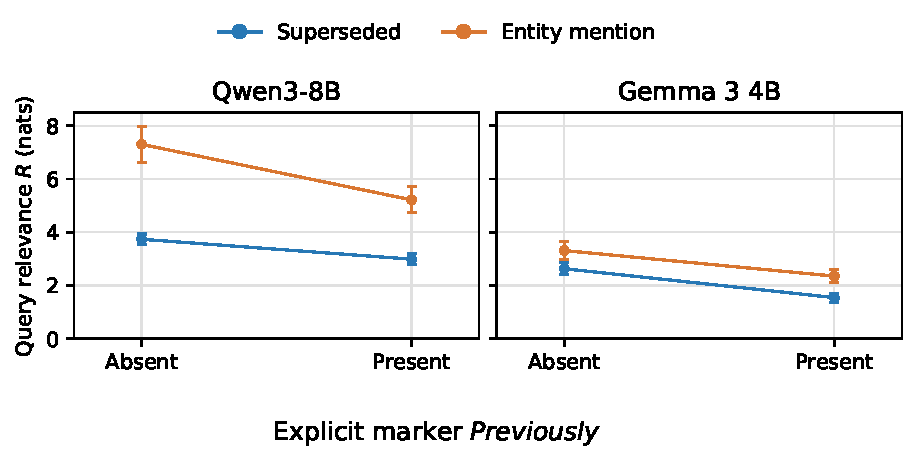
\includegraphics[width=0.9\linewidth]{figures/marker_by_construction.pdf}
\end{center}
\caption{Query relevance in Experiment 2 by marker and construction, separately for aligned (top) and reversed (bottom) order. Points are means over 96 histories; intervals are marginal 95\% history-bootstrap intervals. In Gemma the lines are further apart without the marker under aligned order and converge under reversed order, so the marker-by-construction interaction changes sign between order groups; paired marker effects and interactions are in Table~\ref{tab:marker}.}
\label{fig:marker-effects}
\end{figure}

\subsection{Query relevance and its components}

$E$ can be split into the change in the donor's score minus the change in the source's score. Applying the $R$ transformation to each part gives $R=R_{\text{donor}}-R_{\text{source}}$. Table~\ref{tab:d-decomposition} reports $R$ and both components in the 96-history run. With the marker, the donor component is smaller and the source component less negative, at the mean level, in both constructions and both models.

\begin{table}[h]
\caption{Overall $R$ and its donor and source components by construction and marker state in the 96-history run (nats).}
\label{tab:d-decomposition}
\begin{center}
\footnotesize
\begin{tabular}{@{}lllrrr@{}}
\toprule
Model & Construction & \lit{Previously} & $R$ & Donor component & Source component \\
\midrule
Qwen3-8B & Superseded & Absent & 3.486 [3.357, 3.628] & 1.622 [1.443, 1.810] & −1.864 [−2.075, −1.654] \\
Qwen3-8B & Superseded & Present & 2.834 [2.721, 2.946] & 1.448 [1.274, 1.621] & −1.386 [−1.581, −1.199] \\
Qwen3-8B & Entity mention & Absent & 6.545 [6.250, 6.866] & 3.106 [2.849, 3.363] & −3.438 [−3.743, −3.166] \\
Qwen3-8B & Entity mention & Present & 4.810 [4.619, 5.015] & 2.281 [2.087, 2.493] & −2.530 [−2.719, −2.345] \\
\midrule
Gemma 3 4B & Superseded & Absent & 2.502 [2.351, 2.663] & 1.244 [1.115, 1.374] & −1.258 [−1.425, −1.097] \\
Gemma 3 4B & Superseded & Present & 1.552 [1.453, 1.654] & 0.793 [0.666, 0.925] & −0.759 [−0.893, −0.620] \\
Gemma 3 4B & Entity mention & Absent & 3.409 [3.252, 3.575] & 1.633 [1.483, 1.783] & −1.776 [−1.935, −1.619] \\
Gemma 3 4B & Entity mention & Present & 2.334 [2.204, 2.474] & 1.104 [0.976, 1.246] & −1.230 [−1.373, −1.080] \\
\bottomrule
\end{tabular}
\end{center}
\end{table}

\subsection{The earlier 24-history run}

The 24-history run gave the same pattern as the 96-history run (Table~\ref{tab:d-marker24}): every marker effect is negative, Qwen's interaction is positive, and Gemma's interaction interval includes zero. Its $R$ decomposition and paired component changes are in Tables~\ref{tab:d-decomposition24} and~\ref{tab:d-paired}. The two runs are not pooled.

\begin{table}[h]
\caption{Marker effects and marker-by-construction interaction in the 24-history run (nats; 95\% history-bootstrap intervals).}
\label{tab:d-marker24}
\begin{center}
\small
\begin{tabular}{@{}llrrr@{}}
\toprule
Model & Order & Superseded & Entity mention & Interaction \\
\midrule
Qwen3-8B & All & −0.750 [−0.917, −0.590] & −2.087 [−2.410, −1.772] & 1.337 [0.976, 1.712] \\
Qwen3-8B & Aligned & −0.372 [−0.552, −0.187] & −1.298 [−1.580, −0.979] & 0.926 [0.581, 1.274] \\
Qwen3-8B & Reversed & −1.127 [−1.324, −0.939] & −2.876 [−3.354, −2.429] & 1.749 [1.236, 2.274] \\
\midrule
Gemma 3 4B & All & −1.085 [−1.308, −0.864] & −0.960 [−1.183, −0.727] & −0.125 [−0.390, 0.136] \\
Gemma 3 4B & Aligned & −1.100 [−1.359, −0.851] & −1.155 [−1.384, −0.915] & 0.055 [−0.233, 0.328] \\
Gemma 3 4B & Reversed & −1.069 [−1.372, −0.785] & −0.765 [−1.123, −0.387] & −0.304 [−0.753, 0.116] \\
\bottomrule
\end{tabular}
\end{center}
\end{table}

\begin{table}[h]
\caption{Overall $R$ and its donor and source components by construction and marker state in the 24-history run (nats).}
\label{tab:d-decomposition24}
\begin{center}
\footnotesize
\begin{tabular}{@{}lllrrr@{}}
\toprule
Model & Construction & \lit{Previously} & $R$ & Donor component & Source component \\
\midrule
Qwen3-8B & Superseded & Absent & 3.738 [3.536, 3.934] & 1.590 [1.118, 2.005] & −2.149 [−2.623, −1.705] \\
Qwen3-8B & Superseded & Present & 2.989 [2.791, 3.186] & 1.283 [0.832, 1.746] & −1.705 [−2.151, −1.242] \\
Qwen3-8B & Entity mention & Absent & 7.304 [6.629, 7.966] & 3.875 [3.477, 4.277] & −3.429 [−4.135, −2.764] \\
Qwen3-8B & Entity mention & Present & 5.217 [4.749, 5.705] & 2.540 [2.171, 2.917] & −2.677 [−3.193, −2.165] \\
\midrule
Gemma 3 4B & Superseded & Absent & 2.631 [2.409, 2.863] & 1.413 [1.170, 1.652] & −1.218 [−1.501, −0.934] \\
Gemma 3 4B & Superseded & Present & 1.546 [1.379, 1.714] & 0.685 [0.445, 0.932] & −0.861 [−1.115, −0.610] \\
Gemma 3 4B & Entity mention & Absent & 3.313 [2.975, 3.669] & 1.732 [1.427, 2.048] & −1.582 [−1.915, −1.276] \\
Gemma 3 4B & Entity mention & Present & 2.353 [2.114, 2.605] & 1.079 [0.874, 1.287] & −1.274 [−1.468, −1.068] \\
\bottomrule
\end{tabular}
\end{center}
\end{table}

\begin{table}[h]
\caption{Paired marker-induced changes (present minus absent) in the donor and source components in the 24-history run (nats); $\Delta R=\Delta R_{\text{donor}}-\Delta R_{\text{source}}$.}
\label{tab:d-paired}
\begin{center}
\small
\begin{tabular}{@{}lllrr@{}}
\toprule
Model & Order & Construction & $\Delta$ donor component & $\Delta$ source component \\
\midrule
Qwen3-8B & All & Superseded & −0.306 [−0.812, 0.237] & 0.443 [−0.100, 1.040] \\
Qwen3-8B & All & Entity mention & −1.335 [−1.640, −1.013] & 0.752 [0.323, 1.140] \\
Qwen3-8B & Aligned & Superseded & −0.286 [−0.840, 0.267] & 0.086 [−0.522, 0.704] \\
Qwen3-8B & Aligned & Entity mention & −0.810 [−1.328, −0.330] & 0.488 [−0.179, 1.070] \\
Qwen3-8B & Reversed & Superseded & −0.327 [−0.995, 0.399] & 0.800 [0.088, 1.557] \\
Qwen3-8B & Reversed & Entity mention & −1.859 [−2.283, −1.435] & 1.017 [0.480, 1.492] \\
\midrule
Gemma 3 4B & All & Superseded & −0.727 [−1.046, −0.420] & 0.357 [−0.009, 0.720] \\
Gemma 3 4B & All & Entity mention & −0.653 [−1.003, −0.310] & 0.307 [−0.021, 0.645] \\
Gemma 3 4B & Aligned & Superseded & −0.547 [−1.049, −0.015] & 0.553 [0.062, 1.085] \\
Gemma 3 4B & Aligned & Entity mention & −0.679 [−1.101, −0.245] & 0.475 [0.056, 0.909] \\
Gemma 3 4B & Reversed & Superseded & −0.907 [−1.298, −0.486] & 0.162 [−0.301, 0.629] \\
Gemma 3 4B & Reversed & Entity mention & −0.626 [−1.085, −0.207] & 0.139 [−0.285, 0.532] \\
\bottomrule
\end{tabular}
\end{center}
\end{table}

\subsection{Exploratory Phi-4-mini extension}

For Phi-4-mini, adding the explicit prefix \lit{Previously,} changed $R$ in the superseded construction by −1.355 nats (95\% CI [−1.561, −1.138]), from 5.146 [4.947, 5.362] without the marker to 3.791 [3.592, 4.004] with it. In the entity-mention construction, the marker effect was 0.145 [−0.018, 0.310], an unresolved change from 4.808 [4.557, 5.107] to 4.953 [4.677, 5.269]. The paired marker-by-construction interaction was −1.500 [−1.734, −1.264], indicating a larger reduction for the superseded construction in this model.

The order-stratified estimates show additional heterogeneity. Superseded marker effects were −1.227 [−1.412, −1.026] in aligned order and −1.483 [−1.758, −1.194] in reversed order. Entity-mention effects were −0.253 [−0.450, −0.059] aligned and 0.544 [0.384, 0.703] reversed. The corresponding interaction was −0.973 [−1.221, −0.714] aligned and −2.027 [−2.330, −1.725] reversed. These exploratory estimates indicate construction- and order-dependent score effects for Phi-4-mini; they do not establish a general model-family pattern or identify a mechanism. They are effects of adding the literal prefix, not evidence of active suppression. No answer-generation accuracy was collected in this candidate-scoring run.

\begin{table}[h]
\caption{Exploratory Phi-4-mini marker-confirmation estimates (nats; 24 histories; 95\% history-bootstrap intervals). Marker effect is present minus absent; interaction is the superseded marker effect minus the entity-mention marker effect.}
\label{tab:d-phi-marker}
\begin{center}
\small
\begin{tabular}{@{}lrrr@{}}
\toprule
Order & Superseded marker effect & Entity-mention marker effect & Interaction \\
\midrule
All & −1.355 [−1.561, −1.138] & 0.145 [−0.018, 0.310] & −1.500 [−1.734, −1.264] \\
Aligned & −1.227 [−1.412, −1.026] & −0.253 [−0.450, −0.059] & −0.973 [−1.221, −0.714] \\
Reversed & −1.483 [−1.758, −1.194] & 0.544 [0.384, 0.703] & −2.027 [−2.330, −1.725] \\
\bottomrule
\end{tabular}
\end{center}
\end{table}

\FloatBarrier

\section{An attempt to lower accuracy with distractors}
\label{app:harder}

Because both models answer at ceiling, we tried to make the task harder by adding distractor entities to the Experiment 1 constructions. Each distractor contributed its own \lit{Previously} line and \lit{Currently} line for the target attribute, with values from a separate vocabulary. The plan was to choose, on development data, the hardest of three levels (2, 4, or 6 distractors) at which Qwen's accuracy on generated answers fell between 65\% and 90\%, and then to test whether edits to the earlier value change generated answers. Before the development results were available, we added a stopping rule: if Qwen exceeded 90\% at all three levels, the study would stop without a test.

Each development level used 12 matched target histories and 1,536 scored prompt members (1,152 unique prompts) per model, with greedy decoding and exact matching of the answer. Prompt members include repeated renderings across paired cells; the three levels are matched development conditions, not independent replications. Qwen exceeded 90\% at every level (Table~\ref{tab:e-accuracy}), so the prespecified stopping rule ended the study: no level was selected and no test data were generated. Gemma was also near ceiling and is not an informative behavioral replication. Qwen's few source-value responses occurred in reversed-order entity-mention controls, where the queried attribute had not been assigned that value; they are not stale-assignment errors. The superseded construction made up a quarter of the prompts (384 per level and model, 1,152 across the three levels), and Qwen and Gemma answered every one of them with the current value, never with the earlier one.

Phi-4-mini was also scored on the same three development datasets as an additional, exploratory model; it was not part of the prespecified level-selection rule. Its exact-match accuracy was 8/1,536 (0.52\%), 38/1,536 (2.47\%), and 66/1,536 (4.30\%) at 2, 4, and 6 distractors. These rates are dominated by response-format failures: in a post hoc string-prefix diagnostic, respectively 1,516, 1,530, and 1,527 outputs began with the expected candidate label, but continued with extra text and therefore remained incorrect under the exact-answer parser. The prefix diagnostic is descriptive and does not redefine correctness. Phi's strict accuracy cannot be interpreted as a response to increasing distractor difficulty, and its floor-level exact-match outcomes do not provide an informative behavioral replication. No Phi test was generated.

This was a limited difficulty manipulation. Distractors used a separate vocabulary and were appended after the target blocks; each distractor's historical and current assignment lines were adjacent. The results show that this specific manipulation did not create the intended difficulty for Qwen. They do not establish robustness to long, crowded, or conflicting contexts generally.

\begin{table}[h]
\caption{Strict exact-match accuracy of generated answers in the distractor development runs, by number of distractor entities.}
\label{tab:e-accuracy}
\begin{center}
\small
\begin{tabular}{@{}lrrr@{}}
\toprule
Model & 2 distractors & 4 distractors & 6 distractors \\
\midrule
Qwen3-8B & 1,531/1,536 (99.67\%) & 1,532/1,536 (99.74\%) & 1,533/1,536 (99.80\%) \\
Gemma 3 4B & 1,534/1,536 (99.87\%) & 1,532/1,536 (99.74\%) & 1,532/1,536 (99.74\%) \\
Phi-4-mini & 8/1,536 (0.52\%) & 38/1,536 (2.47\%) & 66/1,536 (4.30\%) \\
\bottomrule
\end{tabular}
\end{center}
\end{table}

\FloatBarrier

\section{Follow-up experiment details}
\label{app:followups}

The follow-ups of Section~\ref{sec:followup-design} were run on the RTX 5080 used for the main experiments, with the same pinned checkpoints, int8 configurations, and scoring code. Each design document was hash-stamped on the experiment machine before its data were generated (not committed to version control; Section~\ref{sec:inference}). Artifact hashes are listed in the supplementary material.

\subsection{Name--value distance}

\paragraph{Choice of the near superseded template.} The design listed three near superseded wordings (\lit{Nora's badge: amber}, \lit{Nora's badge = amber}, \lit{Nora's badge, amber}) and a rule choosing the first whose baseline/edit pairs differ only in the edited value's tokens for both tokenizers. A tokenizer audit run before data generation found that all three pass that check but leave the measured name--value gap unchanged (three tokens in Qwen, four in Gemma, as for the far template), so the superseded arm would not have varied distance. Before any data were generated, an amendment added a fourth candidate, \lit{Previously, the badge of Nora was amber.}, and required the chosen template to be measurably nearer than the far template in both tokenizers; the re-run audit chose it, with a gap of one token in both. The amendment was hash-stamped separately.

\paragraph{Data.} 96 histories (Experiment 1's allocation of entity pairs, attributes, and name orientations), excluding all histories of the marker pilot and the 24-history marker run; 12,288 scored prompts per model (9,152 distinct); scoring took 6,472 s (Qwen) and 2,656 s (Gemma). Results are in Table~\ref{tab:distance}; the distance-by-construction interaction (superseded near-minus-far minus entity-mention near-minus-far) was 0.871 [0.703, 1.040] in Qwen and 0.420 [0.291, 0.542] in Gemma.

\subsection{Update chains}

\paragraph{Vocabulary.} Disjoint chains of up to five values per entity plus two donors need twelve values. The design extended the eight-value vocabulary by walking a recorded candidate list in order and keeping each value that is not a substring of another and keeps the candidate continuations valid for both tokenizers; the audit kept the first four candidates, \lit{olive}, \lit{plum}, \lit{navy}, and \lit{rust}.

\paragraph{Development.} 12 histories per depth (32 prompts per history: historical order $\times$ current order $\times$ edited entity $\times$ query $\times$ baseline/edit), greedy decoding with at most 32 new tokens, and the exact-answer parser of Appendix~\ref{app:harder}. Table~\ref{tab:f-chains} reports accuracy, the share of answers naming any earlier value, and $R$ from candidate masses over the twelve values. Every answer was correct for both models at every depth, so the recorded selection rule chose no depth and the confirmation was not generated.

\begin{table}[h]
\caption{Update-chain development runs (12 histories, 384 generated answers per depth and model). Accuracy is exact-match accuracy of generated answers; ``earlier value'' is the share of answers naming any superseded value; $R$ is mean query relevance from candidate masses.}
\label{tab:f-chains}
\begin{center}
\small
\begin{tabular}{@{}llrrr@{}}
\toprule
Model & Depth & Accuracy & Earlier value & $R$ (nats) \\
\midrule
Qwen3-8B & 3 & 384/384 & 0 & 7.940 \\
Qwen3-8B & 4 & 384/384 & 0 & 10.612 \\
Qwen3-8B & 5 & 384/384 & 0 & 12.040 \\
\midrule
Gemma 3 4B & 3 & 384/384 & 0 & 3.345 \\
Gemma 3 4B & 4 & 384/384 & 0 & 3.289 \\
Gemma 3 4B & 5 & 384/384 & 0 & 3.674 \\
\bottomrule
\end{tabular}
\end{center}
\end{table}

\paragraph{Candidate-score run.} Because no depth qualified for a generation confirmation, a second run scored candidate masses only on 96 fresh histories per depth (dataset seed 20261110; development histories excluded). Table~\ref{tab:f-chains96} gives $R$ by depth and the depth differences, compared across independent history sets by resampling each set separately.

\begin{table}[h]
\caption{Update chains, candidate-score run (96 histories per depth). $R$ in nats with 95\% history-bootstrap intervals; depth differences use independent-set bootstrap intervals.}
\label{tab:f-chains96}
\begin{center}
\small
\begin{tabular}{@{}lrr@{}}
\toprule
 & Qwen3-8B & Gemma 3 4B \\
\midrule
$R$, depth 3 & 7.353 [6.972, 7.725] & 3.450 [3.229, 3.676] \\
$R$, depth 4 & 10.762 [10.303, 11.220] & 3.462 [3.258, 3.667] \\
$R$, depth 5 & 11.835 [11.424, 12.286] & 3.708 [3.479, 3.936] \\
\midrule
Depth 4 $-$ depth 3 & 3.410 [2.835, 3.969] & 0.012 [−0.297, 0.305] \\
Depth 5 $-$ depth 4 & 1.072 [0.469, 1.680] & 0.246 [−0.050, 0.552] \\
Depth 5 $-$ depth 3 & 4.482 [3.915, 5.047] & 0.258 [−0.063, 0.557] \\
\bottomrule
\end{tabular}
\end{center}
\end{table}

\subsection{Updated other attribute}

The 96 histories follow Experiment 1's allocation; the other attribute and the filler attribute are \lit{team} and \lit{project}, swapped between the two halves of the histories, and each history uses all eight vocabulary values (two historical, two extra current, two current for the queried attribute, two donors). Historical order, current order, edited entity, query, and baseline/edit are crossed as in Experiment 1, with the extra current block in the current order; 9,216 prompts per model (6,912 distinct). By order group, the queried-attribute effect was 0.801 [0.691, 0.919] (aligned) and 0.679 [0.579, 0.780] (reversed) in Qwen and 0.362 [0.205, 0.528] and −0.066 [−0.198, 0.064] in Gemma; the update effect was −0.225 [−0.334, −0.117] and −0.354 [−0.452, −0.249] in Qwen and −0.036 [−0.186, 0.099] and −0.019 [−0.150, 0.118] in Gemma.

\subsection{Additional models}

\paragraph{Procedure.} Each additional model was scored on Experiment 1's sealed screening dataset (24 histories) and, if it passed, on the sealed confirmation dataset (96 histories), with the same renderer, candidate validation, scorer, competence rule, and analysis code as Qwen and Gemma. Llama-3.1-8B-Instruct, the planned model from a third family, could not be used because access to its gated weights was declined. Qwen3-14B ran out of memory while loading with int8 weights on the 16 GB GPU and produced no scores.

\paragraph{Screens.} Table~\ref{tab:f-screens} gives strict rank-one accuracy on distinct screening prompts. OLMo-2-7B-Instruct (revision \lit{470b1fba1ae01581f270116362ee4aa1b97f4c84}, int8 weights, bfloat16 computation) failed in four constructions. Phi-4-mini, re-scored with this procedure, reproduced its original screening result exactly.

\begin{table}[h]
\caption{Competence screens of the additional models: correct current value strictly ranked first, over distinct screening prompts (requirement: 99\% in every construction).}
\label{tab:f-screens}
\begin{center}
\small
\begin{tabular}{@{}lrr@{}}
\toprule
Construction & OLMo-2-7B-Instruct & Phi-4-mini \\
\midrule
Live & 287/288 & 288/288 \\
Superseded & 563/576 & 576/576 \\
Other attribute & 575/576 & 573/576 \\
Entity mention & 426/576 & 561/576 \\
Early unassigned & 452/576 & 576/576 \\
Late unassigned & 448/576 & 576/576 \\
\bottomrule
\end{tabular}
\end{center}
\end{table}

\paragraph{Phi-4-mini, descriptive confirmation.} Outside the screen, Phi-4-mini was scored on all 18,432 confirmation prompts. Table~\ref{tab:f-phi} reports its condition-level relevance and the three planned contrasts; they are descriptive.

\begin{table}[h]
\caption{Phi-4-mini on the Experiment 1 confirmation set (descriptive; the model failed the competence screen). Means with 95\% history-bootstrap intervals over 96 histories, in nats.}
\label{tab:f-phi}
\begin{center}
\small
\begin{tabular}{@{}lr@{}}
\toprule
Quantity & Phi-4-mini \\
\midrule
$R$ live & 17.593 [17.223, 17.941] \\
$R$ superseded & 3.110 [2.998, 3.221] \\
$R$ other attribute & 3.262 [3.141, 3.393] \\
$R$ entity mention & 4.982 [4.780, 5.179] \\
$R$ early unassigned & 0.027 [−0.069, 0.130] \\
$R$ late unassigned & −0.000 [−0.117, 0.115] \\
\midrule
Superseded $-$ other attribute & −0.152 [−0.266, −0.040] \\
Superseded $-$ entity mention & −1.872 [−2.091, −1.664] \\
Superseded $-$ early unassigned & 3.082 [2.961, 3.197] \\
\bottomrule
\end{tabular}
\end{center}
\end{table}



\end{document}
